\documentclass[a4paper,12pt]{report}
\usepackage[french]{babel}
\usepackage[utf8]{inputenc}
\usepackage[T1]{fontenc}
\usepackage[pdftex]{graphicx}
\graphicspath{ {images/} }
\usepackage{setspace}   
\usepackage[hidelinks]{hyperref}
\usepackage{lscape}
\usepackage{everypage}
\usepackage{lipsum}
\usepackage{pifont}  % for some special characters 
\usepackage{diagbox}
\usepackage{lmodern}
\usepackage {framed}
\usepackage[acronym]{glossaries}
\makeglossaries
\usepackage[Conny]{fncychap}
\usepackage{float}
\usepackage{amsmath}
\usepackage{graphicx}
\usepackage[table,xcdraw]{xcolor}
\usepackage{url}
\usepackage{array}
\usepackage{fourier, erewhon, cabin}
\usepackage{mathptmx}
\usepackage[colorinlistoftodos]{todonotes}
\usepackage{xspace}
\usepackage[french]{minitoc}
\usepackage{hyperref}
%\fboxsep=1mm%padding thickness
\fboxrule=1pt%border thickness
%pour la mise en page des tableaux
\usepackage{array}
%\usepackage{ulem}
\usepackage{ragged2e}
\justifying
\usepackage{tabularx}
\usepackage{longtable}
\usepackage[top=2cm, bottom=2cm, left=3cm, right=2cm]{geometry}
\usepackage{subfig}
\setlength {\marginparwidth }{2cm} 
\setcounter{secnumdepth}{4}
\setcounter{tocdepth}{4}
\setcounter{minitocdepth}{2}
\mtcsetrules{*}{off}
\mtcsettitle{minitoc}{}
\setstretch{1,5}
\hypersetup{}
\renewcommand{\arraystretch}{1,3}
\newcolumntype{R}[1]{>{\raggedleft\arraybackslash }b{#1}}
\newcolumntype{L}[1]{>{\raggedright\arraybackslash }b{#1}}
\newcolumntype{C}[1]{>{\centering\arraybackslash }b{#1}}
\renewcommand{\figurename}{\textbf{Figure}}
\renewcommand{\tablename}{\textbf{Tableau}}
\addto\captionsfrench{\renewcommand{\bibname}{Netographie \& Bibliographie}}
\addto\captionsfrench{\renewcommand{\glossaryname}{Acronymes}}
\addto\captionsfrench{\renewcommand{\contentsname}{}}
\makeatletter
\renewcommand\tableofcontents{%
  \null\hfill\textbf{\Large\contentsname}\hfill\null\par % line to comment if Glenn style also wanted here
  \@mkboth{\MakeUppercase\contentsname}{\MakeUppercase\contentsname}%
  \@starttoc{toc}%
}
\makeatother
\usepackage{lettrine}
\usepackage{xstring}
\usepackage{multirow}
%%%%
\newacronym{UML}{UML}{Langage de Modélisation Unifié}
\newacronym{BI}{BI}{Busniss intelligence}

%%%%
%======= DEBUT DU DOCUMENT =======
\begin{document}
\newcommand{\HRule}{\rule{\linewidth}{2mm}}
%sous sommaire en francais
\pagenumbering{roman}
\chapter*{Thanks}
I would like to express my deep gratitude for my supervisor for all the help and support. I would also like to extend my thanks to \textbf{Mr. Foued Oueslati} and the teachers of the Higher Institute of for their advice and support during the internship.

\chapter*{Contents} 
\dominitoc  % Initialization du sous sommaire
\tableofcontents
\listoffigures
\listoftables
\printglossaries
%recommencer la numérotation des pages à "1"
\clearpage
\pagenumbering{arabic}
\setcounter{page}{1}
\chapter*{General Introduction}
\addstarredchapter{General Introduction} 
This report describes the work in an internship project carried out within VIPAY SARL.
The objective of the project is to create an instructor dashboard for an e-learning website.
\hfill \break
\hfill \break
In the first part, this document will present VIPAY SARL from which we carried out this project. We will then present the overall description of the project
while emphasizing the different axes on which the instructor dashboard must be
built on. We expose the modeling part for which we used the UML language, and
finally the implementation phase.

\chapter{General overview}
\minitoc
\newpage
\section*{Introduction}
This chapter will you a general overview about the project. We start by presenting the project and analyse the requirements.
\addcontentsline{toc}{section}{Introduction}
\section{Presenting the company}
This project is built for the company VIPAY SARL. I'm one of the interns in the company and
my mission was to build an instructor dashboard for study.tn, an online video based e-learning platform for Tunisia where students can enroll in video based courses, and learn from the best instructors, in their own pace, anywhere, at anytime and in low cost.
\section{Presenting the project}
Study.tn is an e-learning platform : It is a training/education approach that theoretically allows learning without the presence of a physical teacher nearby, 
\hfill \break
\hfill \break
The platform consists of three spaces :

\begin{itemize}
  \item The Student space where students can enroll and watch courses.
  \item The instructor space where the instructor can manage his courses, sales.
  \item The admin space where Study.tn team can manage users and courses 
\end{itemize}

\hfill \break
In this project we will build a new instructor dashboard. In this dashboard the instructor can manage the courses, manage sales and communicate with students.
\section{The existing solutions}
\subsection{Analysis of the existing solutions}
The current study.tn website already has its own instructor dashboard where the instructor can add, delete or edit courses. The instructor can set the general informations such as course title,
sub-title, price, description , category and cover photo. They can add chapters and lectures. Instructors can add requirements and exam questions. They can also check their sales.

\begin{figure}[!ht]
    \centering
    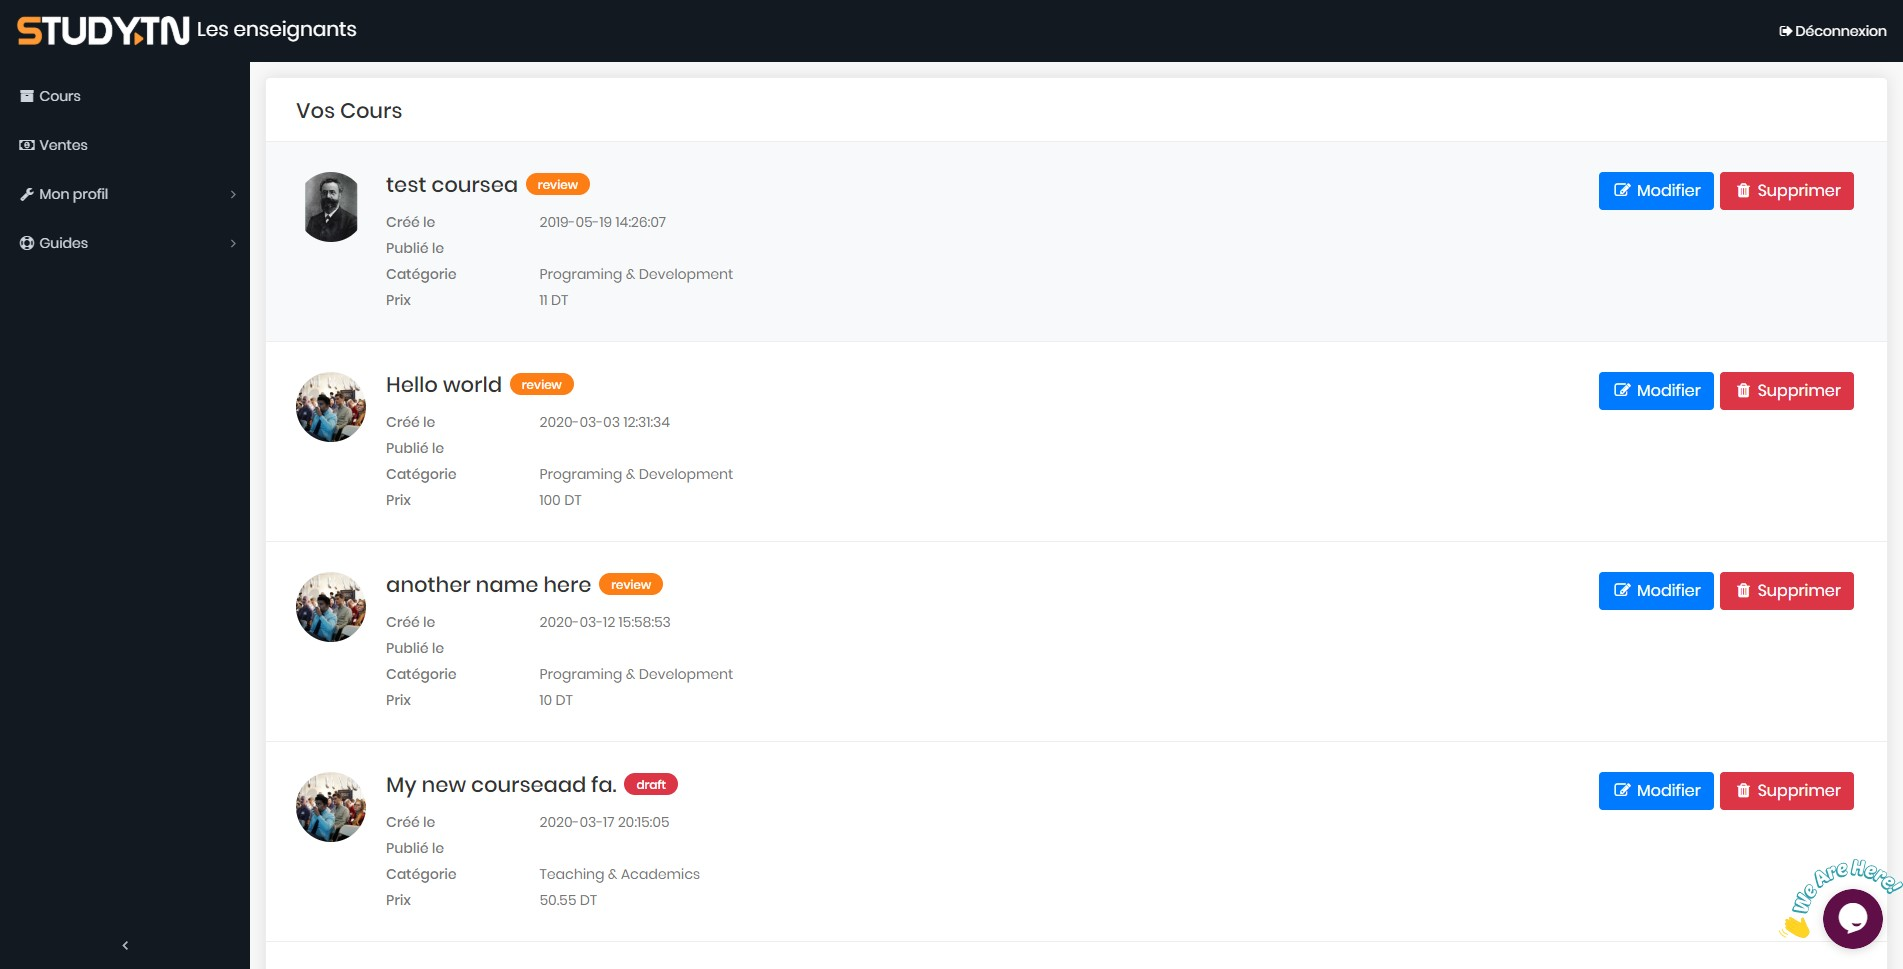
\includegraphics[width=150mm]{currrent_instuctor_space.jpg}
    \caption{The current study.tn instructor dashboard}
    \label{fig:currrent_instuctor_space}
\end{figure}

\subsection{Problem of the existing solutions}
Server-side rendering is a common method for displaying information onto the screen. It works by converting HTML files in the server into usable information for the browser. Whenever you visit a website, your browser makes a request to the server that contains the contents of the website. Once the request is done, your browser will display the rendered HTML on the screen. The current instructor dashboard uses server-side rendering with a template enging which leads to the following issues : 
\hfill \break
\begin{itemize}
  \item Touching the front-end risks touching back-end as in theory you can't do a UI rebuilt without messing backend.
  \item Full page reloads when changing routes.
  \item Frequent server requests which The will increase the load on the server.
  \item An overall slow page rendering as the HTML doc gets bigger.

\end{itemize}

\subsection{Proposed solution}
All of the issues above can be overcomed using a front-end framework. We decided to go with react as it is the most used framework for building large scale web applications. Built by Facebook, React makes it simple to create interactive user interfaces. The framework is designed for building component based applications and with the support of backward compatibility, so you can rest assured of its longevity. React has almost 3 million users and a massive developer community. These are the advantages of using react :

\hfill \break

\begin{itemize}
  \item Does not require page reloading during use.
  \item Only load the data from the server when needed.
  \item Fast page rendering as it only re-render the components that needs to be updated.
\end{itemize}


%fin code item
\section{Project management}

\subsection{Agile method}
An Agile method is carried out in a collaborative spirit and adapt to incremental approaches. It generates high-quality products while taking into account requirement changes. It also allows
to manage quality continuously and detect problems as soon as possible,
thus allowing corrective actions to be taken without too many penalties in the
costs and deadlines. For our project, we focused on a
Agile type method and more particularly SCRUM\cite{cite0}.

\subsection{Why SCRUM}
SCRUM is a project management method that only presents qualities: 

\begin{itemize}
  \item It is mainly focused on quality, objectives, efficiency.
  \item Minimization of bugs while allowing an excellent communication in the project through the daily Scrum meeting.
  \item The tasks and the "reviewing" process in the project are perfectly defined which totally improves progress.
\end{itemize}


\vfill
\clearpage

\begin{figure}[!ht]
    \centering
    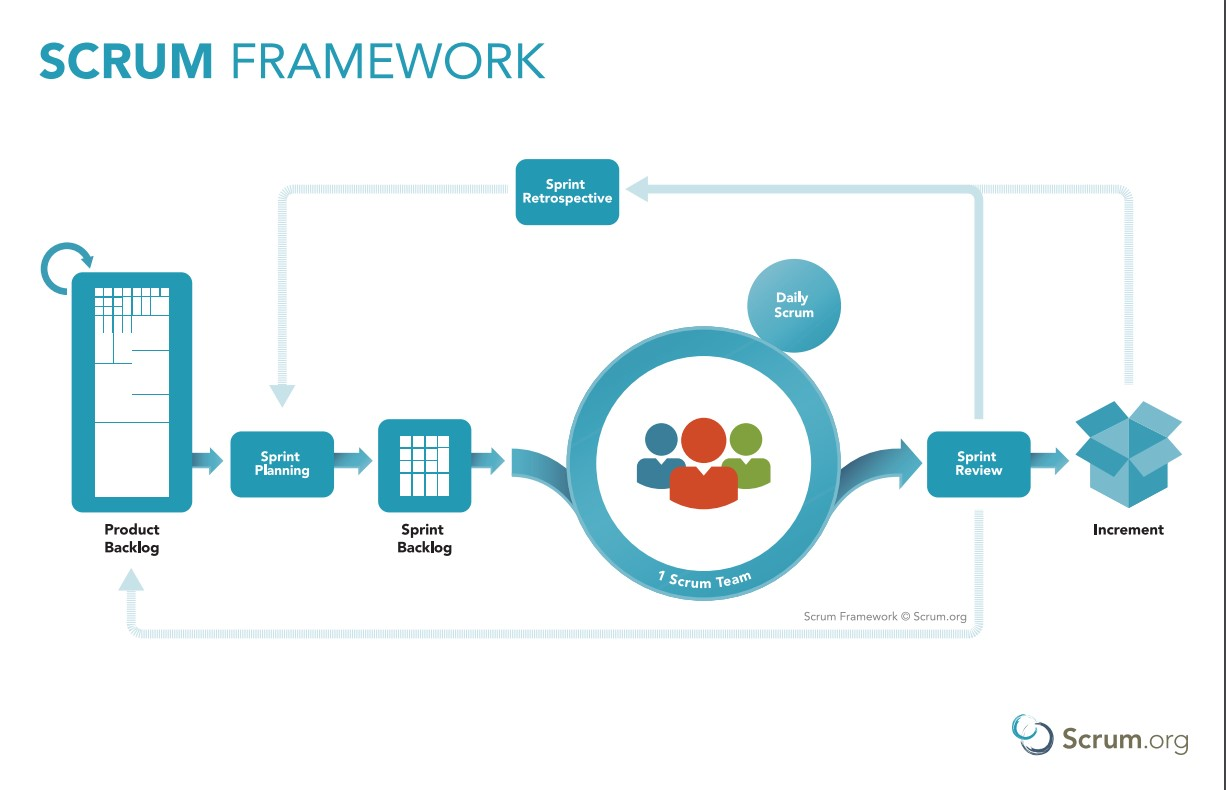
\includegraphics[width=150mm]{scrum.jpg}
    \caption{The Scrum Framework}
    \label{fig:scrum}
\end{figure}



\subsection{UML\cite{cite1}}

UML (Unified Modeling Language) is a formal language normalized in terms of
object modeling.

\subsection{Why UML}
UML brings many advantages such as :
\begin{itemize}
  \item Its independence from programming languages, application and process areas, its versatility and flexibility have made him a universal language.
  \item make the representation and understanding of object solutions easier.
  \item Its graphic notation allows to express an object solution visually, which helps in the comparison and evaluation of solutions.
\end{itemize}

\section*{Conclusion}
In this chapter, we gave a general idea about the company and project.

\addcontentsline{toc}{section}{Conclusion}
%\gls{UML}........\acrshort{UML}
\chapter{Requirements analysis}
\minitoc
\newpage
\section*{Introduction}
\addcontentsline{toc}{section}{Introduction}
\section{Requirements analysis}

\subsection{Use case diagram}

\begin{figure}[!ht]
    \centering
    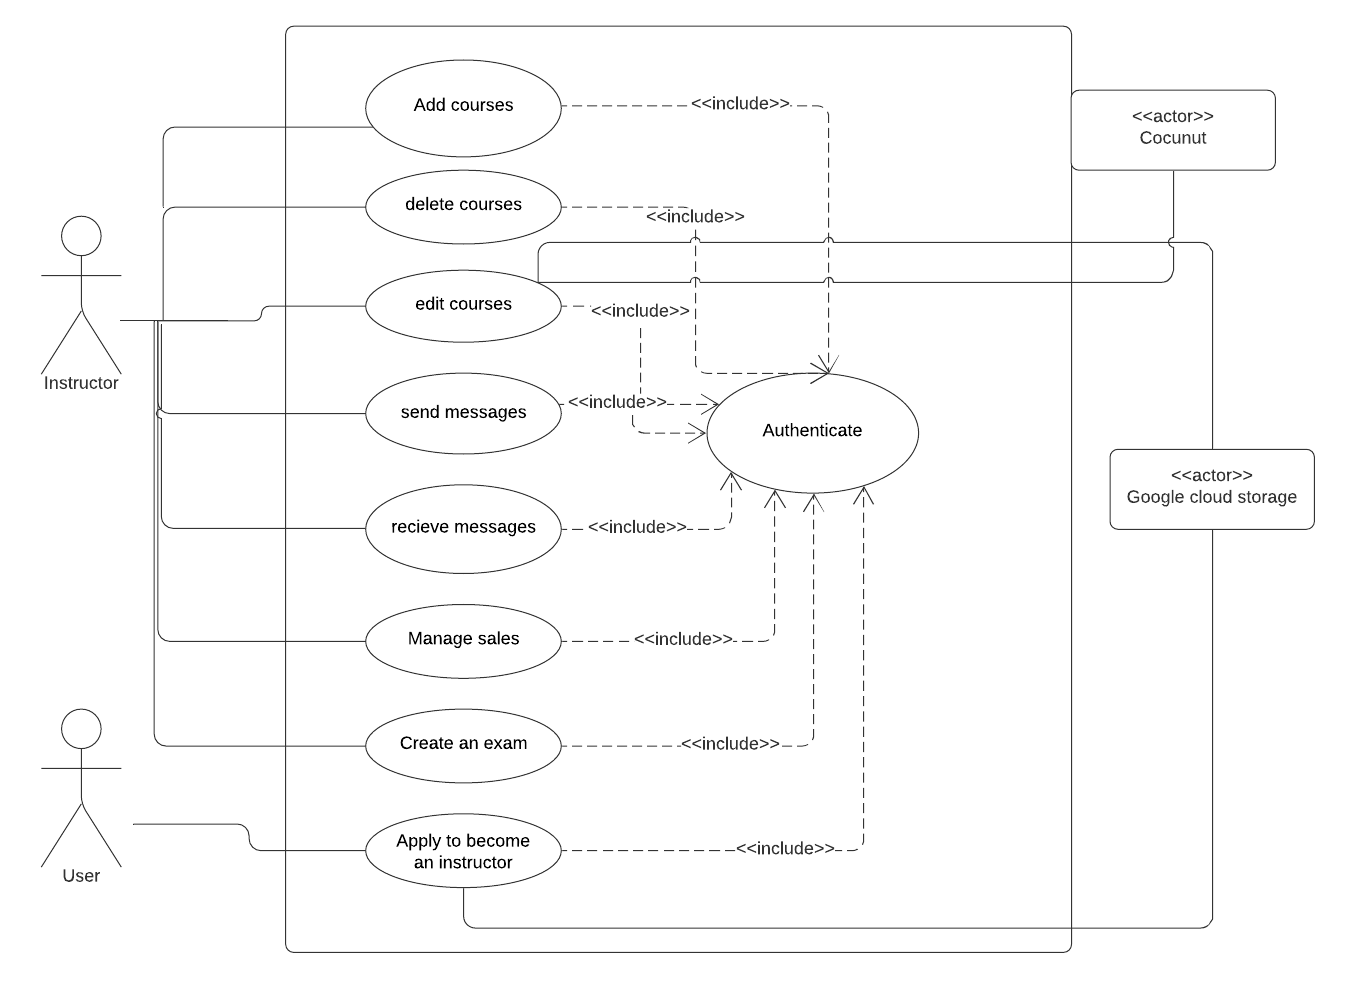
\includegraphics[width=170mm]{use_case.png}
    \caption{Use case diagram}
    \label{fig:use_case}
\end{figure}


\subsection{Use case diagram details}
\hfill \break
\textbf{Coconut :} coconut is the transcoding service that we use to transcode the videos upload.
\hfill \break
\textbf{Google cloud storage :} is the service we where we store the uploaded files and course videos.
\hfill \break
\textbf{Instructor :} is the user of the dashboard instructor.
\hfill \break
\textbf{User :} is a normal user that is not an instructor.
 

\subsection{Database schema}

The figure below shows the database schema that is already built.

\begin{figure}[!ht]
    \centering
    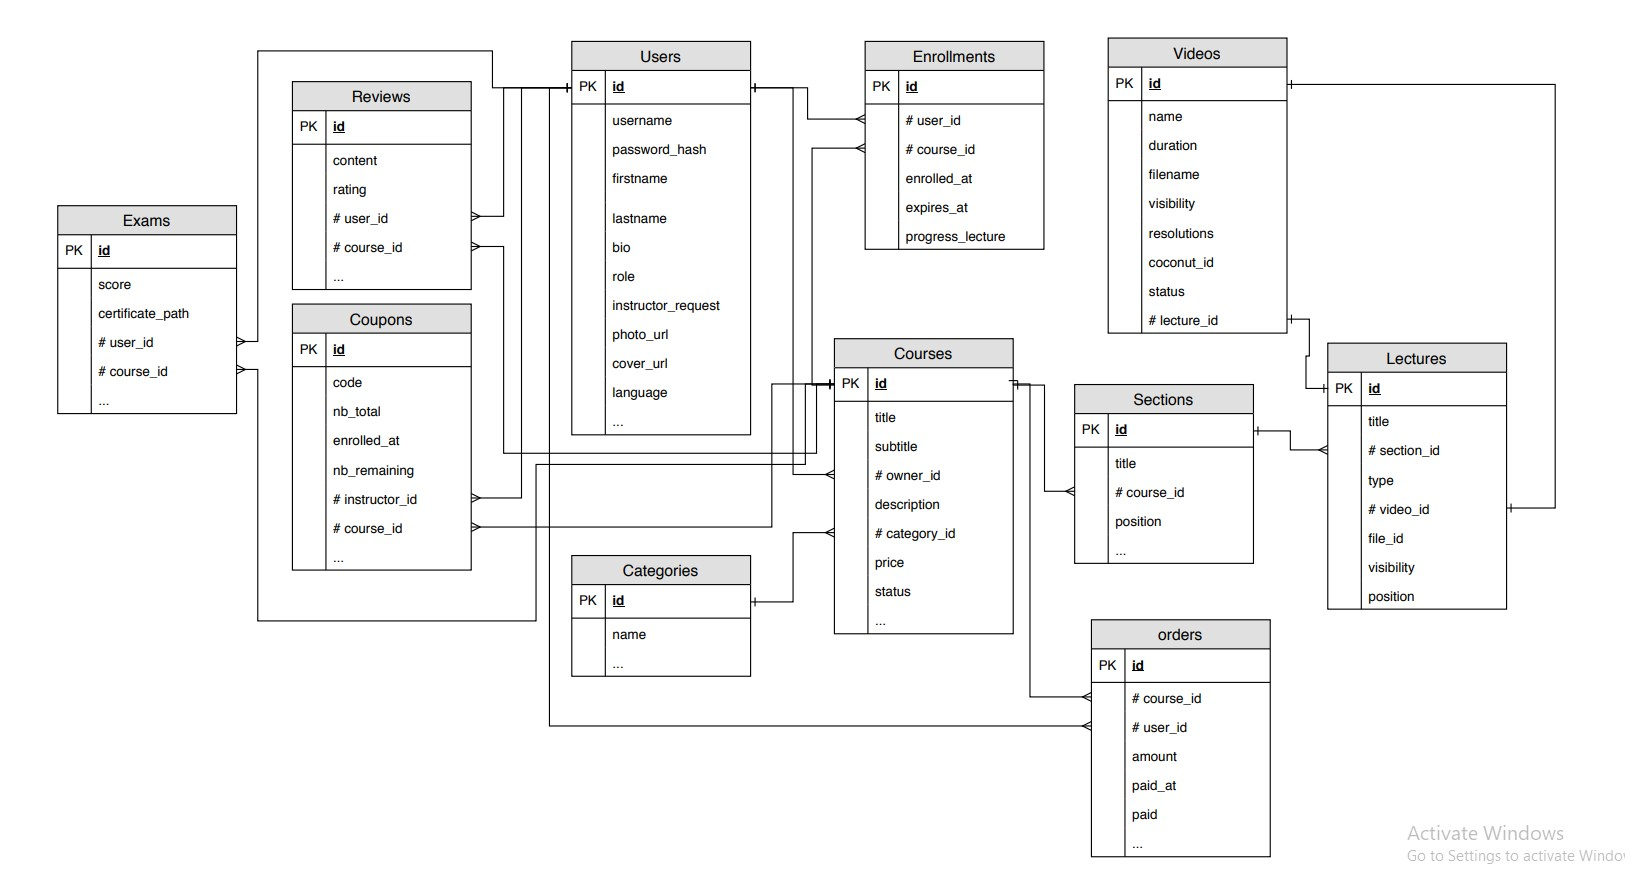
\includegraphics[width=170mm]{database_schema.jpg}
    \caption{Database schema}
    \label{fig:database_schema}
\end{figure}


\subsection{Functional requirements}
\begin{itemize}
    \item[\ding{81}] Instructor must be able to add courses.
    \item[\ding{81}] Instructor must be able to delete courses.
    \item[\ding{81}] Instructor must be able to edit courses.
    \item[\ding{81}] Instructor must be able to send messages to students.
    \item[\ding{81}] Instructor must be able to recieve messages from students.
    \item[\ding{81}] Instructor must be able to see courses sales.
    \item[\ding{81}] Instructor must be able to create an exam.
    \item[\ding{81}] User must be able to apply to become an instructor.
\end{itemize}
\subsection{Non functional requirements}
\begin{itemize}
    \item[\ding{81}] The application must be efficient and have low response time.
    \item[\ding{81}] The application must be secure.
    \item[\ding{81}] The application must be simple to use. The user must not encounter any obstacle or ambiguity during his experience.
\end{itemize}

\section{Prototypes}
This section will show the wireframes created using Adobe xd.

\subsection{Courses tab}

The figure below shows the courses tab where the instructor can see his courses.

\begin{figure}[!ht]
    \centering
    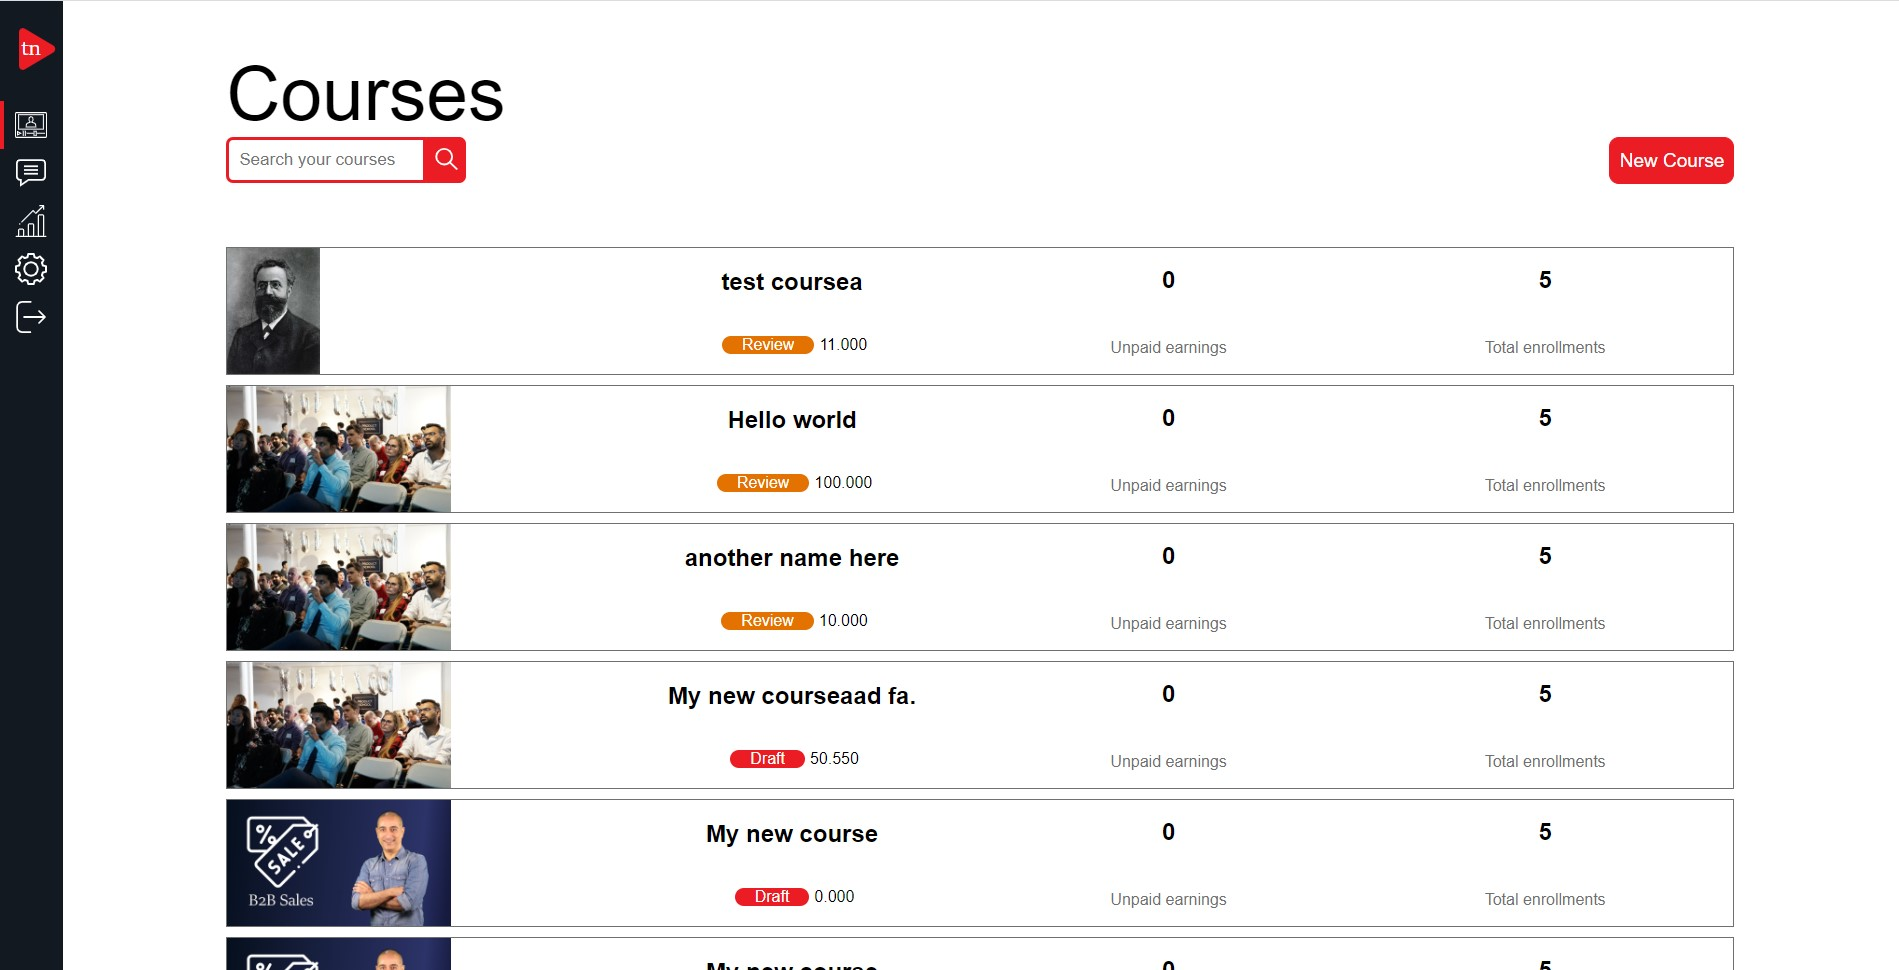
\includegraphics[width=170mm]{courses_tab.jpg}
    \caption{Wireframe for the courses tab}
    \label{fig:courses_tab}
\end{figure}


\vfill
\clearpage

\subsection{Edit course}


The figure below shows the curriculum form where the instructor can add chapters and lectures and attach videos to them.

\begin{figure}[!ht]
    \centering
    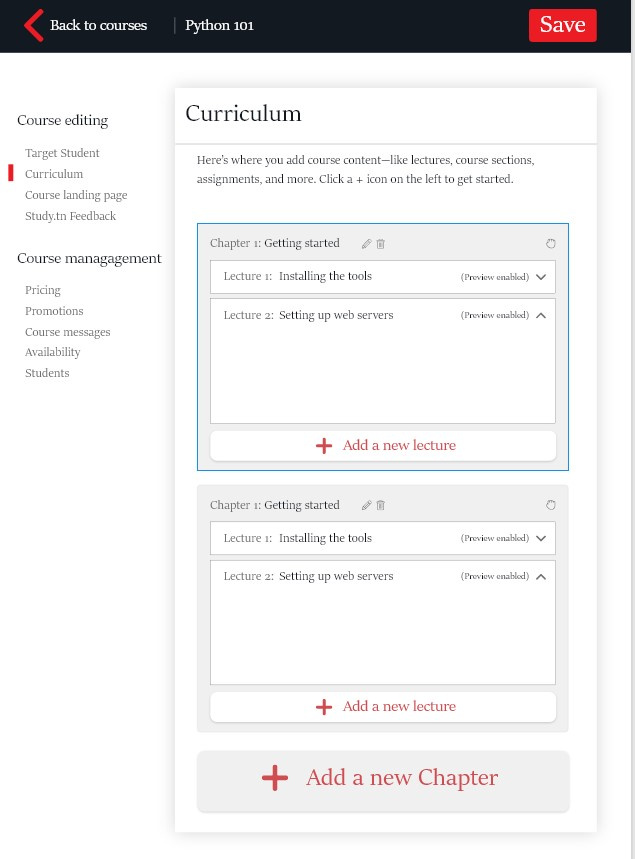
\includegraphics[width=150mm]{edit_course_cir_form.jpg}
    \caption{Wireframe for the curriculum form}
    \label{fig:edit_course_cir_form}
\end{figure}

The figure below shows the landing page form where the instructor can edit the course data like title and description.

\begin{figure}[!ht]
    \centering
    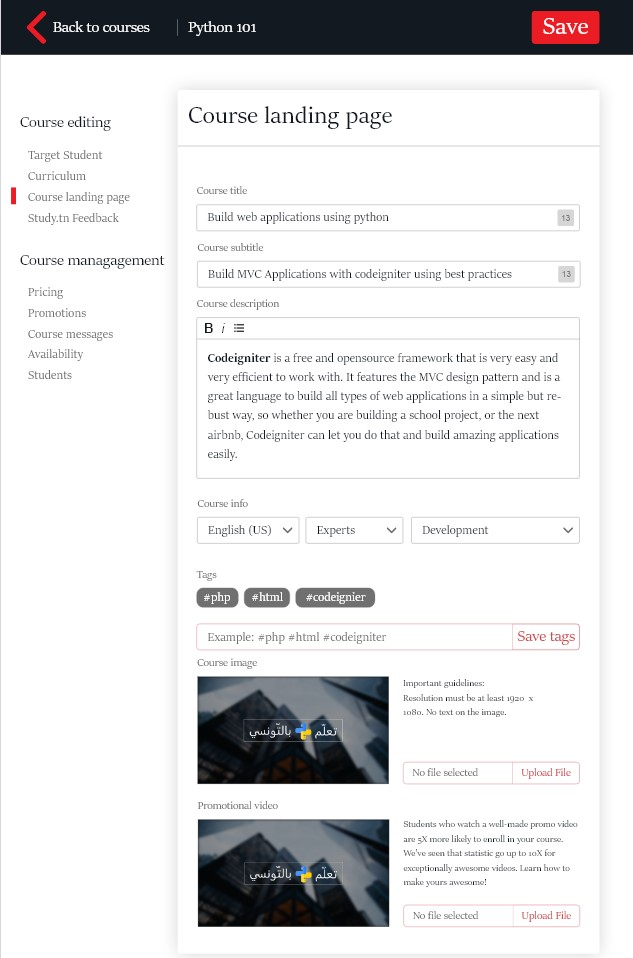
\includegraphics[width=150mm]{edit_course_landing_page_form.jpg}
    \caption{Wireframe for the landing page form}
    \label{fig:edit_course_landing_page_form}
\end{figure}

The figure below shows the pricing form where the instructor can edit his course price.

\begin{figure}[!ht]
    \centering
    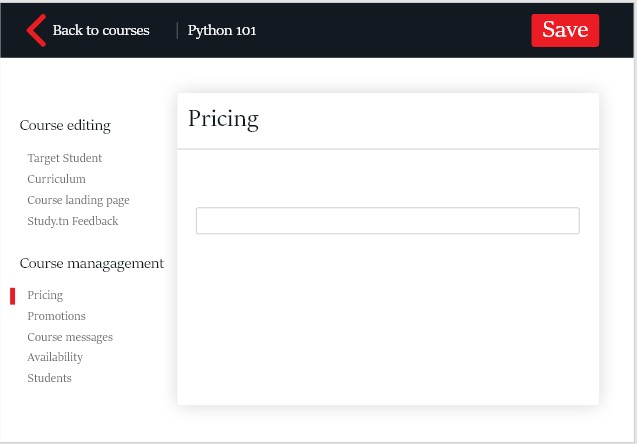
\includegraphics[width=150mm]{edit_course_price.jpg}
    \caption{Wireframe for the price form}
    \label{fig:edit_course_price}
\end{figure}

\vfill
\clearpage

The figure below shows the target students form where the instructor can define the requirements needed before taking the course.

\begin{figure}[!ht]
    \centering
    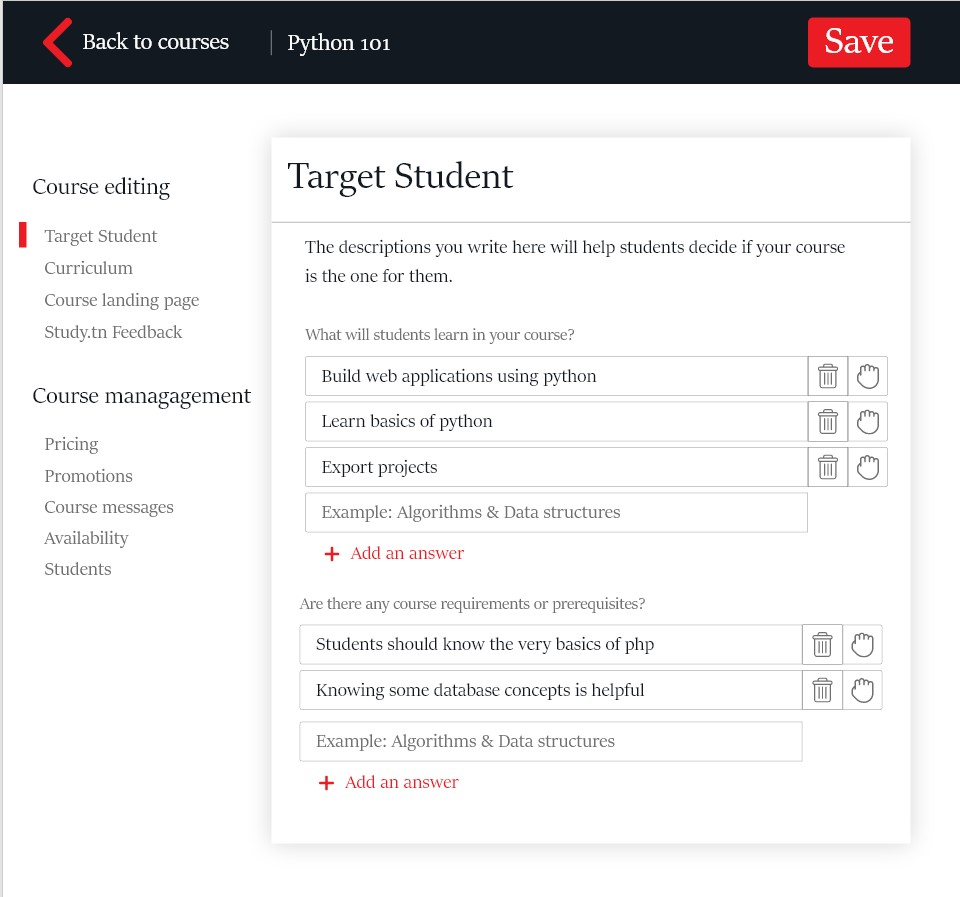
\includegraphics[width=150mm]{edit_course_target_form.jpg}
    \caption{Wireframe for the target students form}
    \label{fig:edit_course_target_form}
\end{figure}

\vfill
\clearpage

\subsection{Communication}

The figures below show the communication part of the dashboard.

\begin{figure}[!ht]
    \centering
    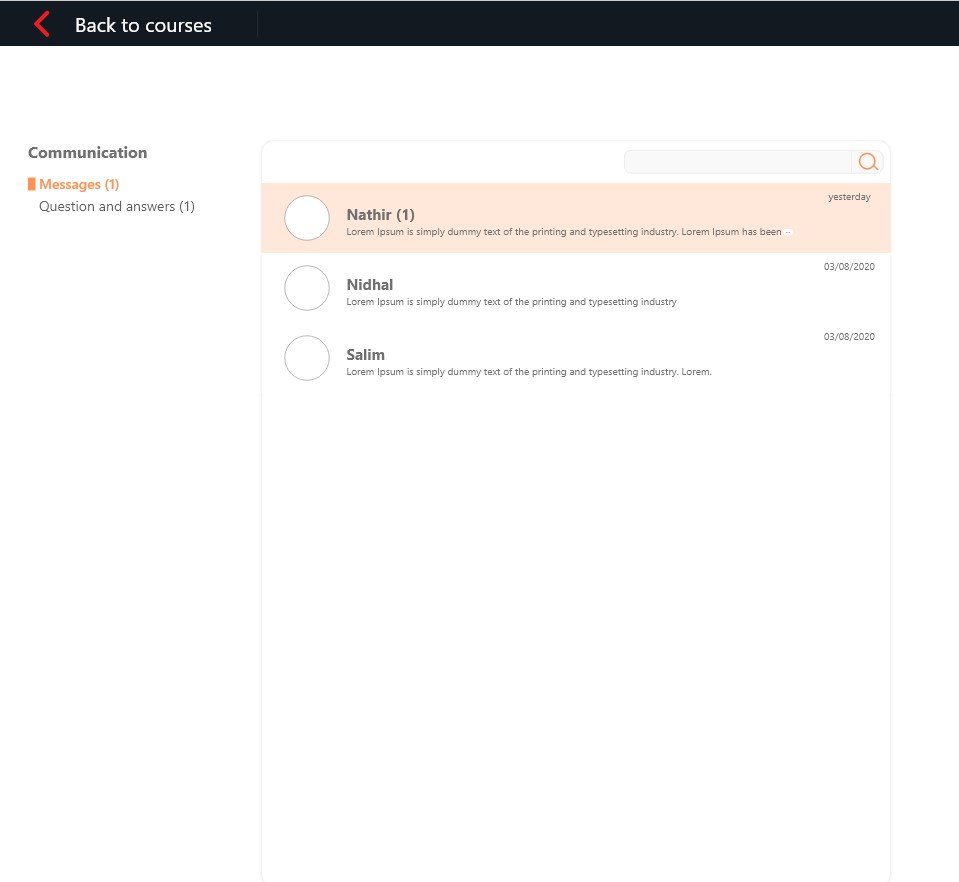
\includegraphics[width=150mm]{conversation_list.jpg}
    \caption{Wireframe for the conversations list}
    \label{fig:conversation_list}
\end{figure}


\vfill
\clearpage

\begin{figure}[!ht]
    \centering
    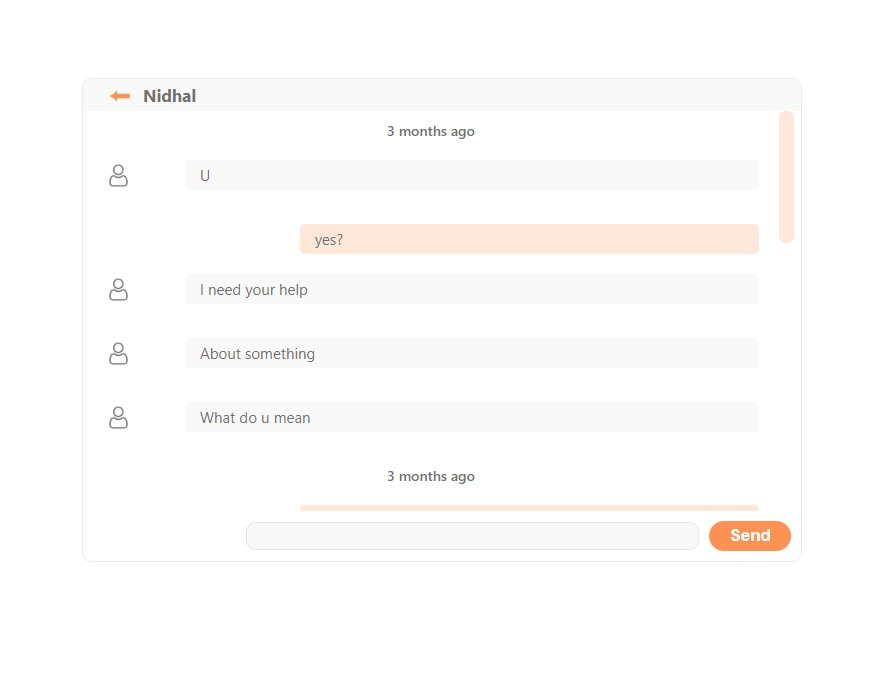
\includegraphics[width=170mm]{conversation.jpg}
    \caption{Wireframe for a conversation}
    \label{fig:conversation}
\end{figure}


\section{Modeling and approach}

\subsection{Product backlog}
%%%%%table
\begin{table}[H]
\centering
\caption{Product backlog}
\begin{tabular}{|p{1cm}|p{1.5cm}|p{3cm}|p{6cm}|p{2cm}|}
\hline
\rowcolor{brown!18}\textbf{\large{ID}} & \textbf{\large{Sprint}} & \textbf{\large{As a}}  & \textbf{\large{I want to be able to}} & \textbf{\large{Priority}} \\
\hline
1& 1 & Instructor & Access the instructor space & High\\\hline
2& 1 & Instructor & Add courses  & High\\\hline
3& 1 & Instructor & Delete my courses  & High\\\hline
4& 1& Instructor & Edit my courses  & High\\\hline
5& 2& Instructor & Send messages to my students & High\\\hline
6& 2& Instructor & Recieve messages from my students  & High\\\hline
7& 2& Instructor  & See my course sales & Normal \\\hline
8& 3& Instructor & Create an exam & High\\\hline
9& 3& User & Apply to become an instuctor  & Normal \\\hline
\end{tabular}
\end{table}



\section*{Conclusion}
\addcontentsline{toc}{section}{Conclusion}
\chapter{Sprint Zero}
\minitoc
\newpage
\section*{Introduction}
This chapter will cover the hardware and software environment the project was built on.
\addcontentsline{toc}{section}{Introduction}
\section{Hardware environment}
The project was built on a desktop computer with the following specs :

\begin{itemize}
  \item Processor : Intel i7-7700 Processor (8M Cache, up to 4.20 GHz)
  \item RAM : 8 GB DDR4 3200 MHZ
  \item Graphic card : GTX  1070 8gb GDDR5
  \item Operating system : GTX  1070 8gb GDDR5
\end{itemize}
\section{Software environment}

\hfill \break
\textbf{React \cite{cite3} :} React is a JavaScript library for building user interfaces. React allows developers to create large web applications that can change data, without reloading the page. The main purpose of React is to be fast, scalable, and simple. It works only on user interfaces in the application. This corresponds to the view in the MVC template.


\textbf{Redux \cite{cite4} :} Redux itself is a standalone library that can be used with any UI layer or framework, including React, Angular, Vue, Ember, and vanilla JS. Although Redux and React are commonly used together, they are independent of each other. It's predictable state container for JavaScript apps.

\hfill \break
\hfill \break
\textbf{Node \cite{cite2} :} Node.js is an open-source, cross-platform, JavaScript runtime environment that executes JavaScript code outside a web browser. Node is required to work with react.

\hfill \break
\hfill \break
\textbf{Adobe XD \cite{cite9} :} XD empowers designers with the speed, precision, and quality to seamlessly iterate and share interactive prototypes with team members and reviewers across devices and platforms, including Windows, Mac, iOS, and Android. We will use that to open and work with the wireframes shown previously.

\vfill
\clearpage

\begin{figure}[!ht]
    \centering
    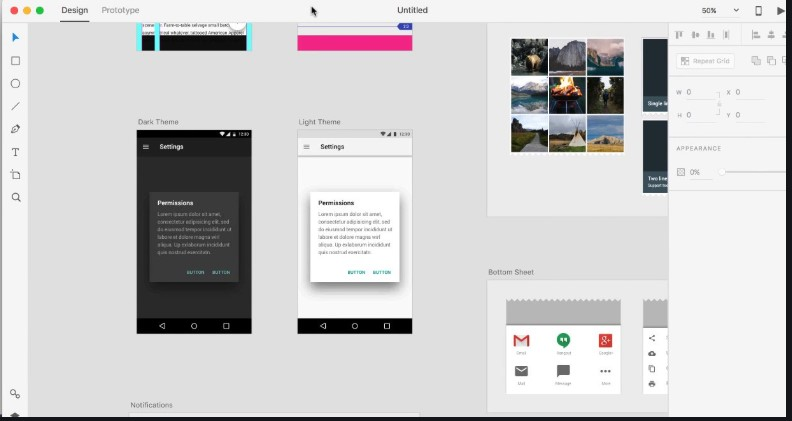
\includegraphics[width=150mm]{adobexd_interface.jpg}
    \caption{Adobe XD interface}
    \label{fig:adobexd_interface}
\end{figure}

\hfill \break
\hfill \break
\textbf{Visual Studio Code \cite{cite7} :} is a code editor developed by Microsoft for Windows, Linux and MacOs. It is one of the best code editors in the market given its speed, the variation of the proposed extensions and the integrated terminal. It also supports several languages and Frameworks such as NodeJS and React.

\begin{figure}[!ht]
    \centering
    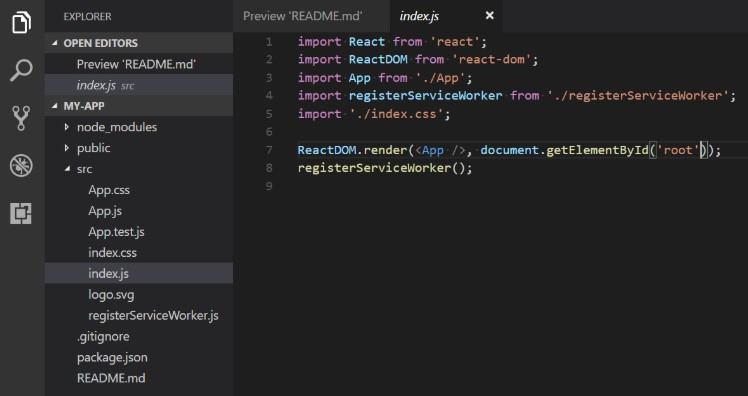
\includegraphics[width=170mm]{visual_code_interface.jpg}
    \caption{Visual Studio interface}
    \label{fig:visual_code_interface}
\end{figure}

\hfill \break
\hfill \break
\textbf{Postman \cite{cite5} :} Postman is a software development tool. It enables people to test calls to APIs. Postman users enter data. The data is sent to a special web server address. Typically, information is returned, which Postman presents to the user.

\begin{figure}[!ht]
    \centering
    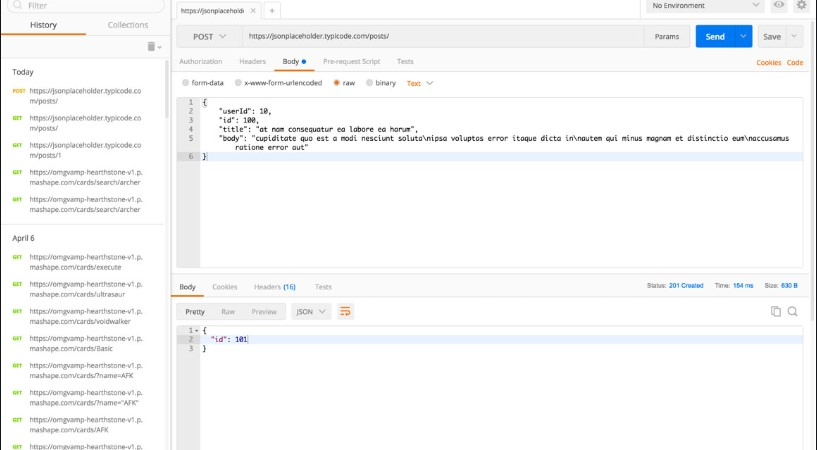
\includegraphics[width=150mm]{postman_interface.jpg}
    \caption{Postman interface}
    \label{fig:postman_interface}
\end{figure}


\hfill \break
\hfill \break
\textbf{Gitlab \cite{cite8} :} is a Git repository hosting service, but it adds many of its own features. While Git is a command line tool, Gitlab provides a Web-based graphical interface. It also provides access control and several collaboration features, such as a wikis and basic task management tools for every project.


\begin{figure}[!ht]
    \centering
    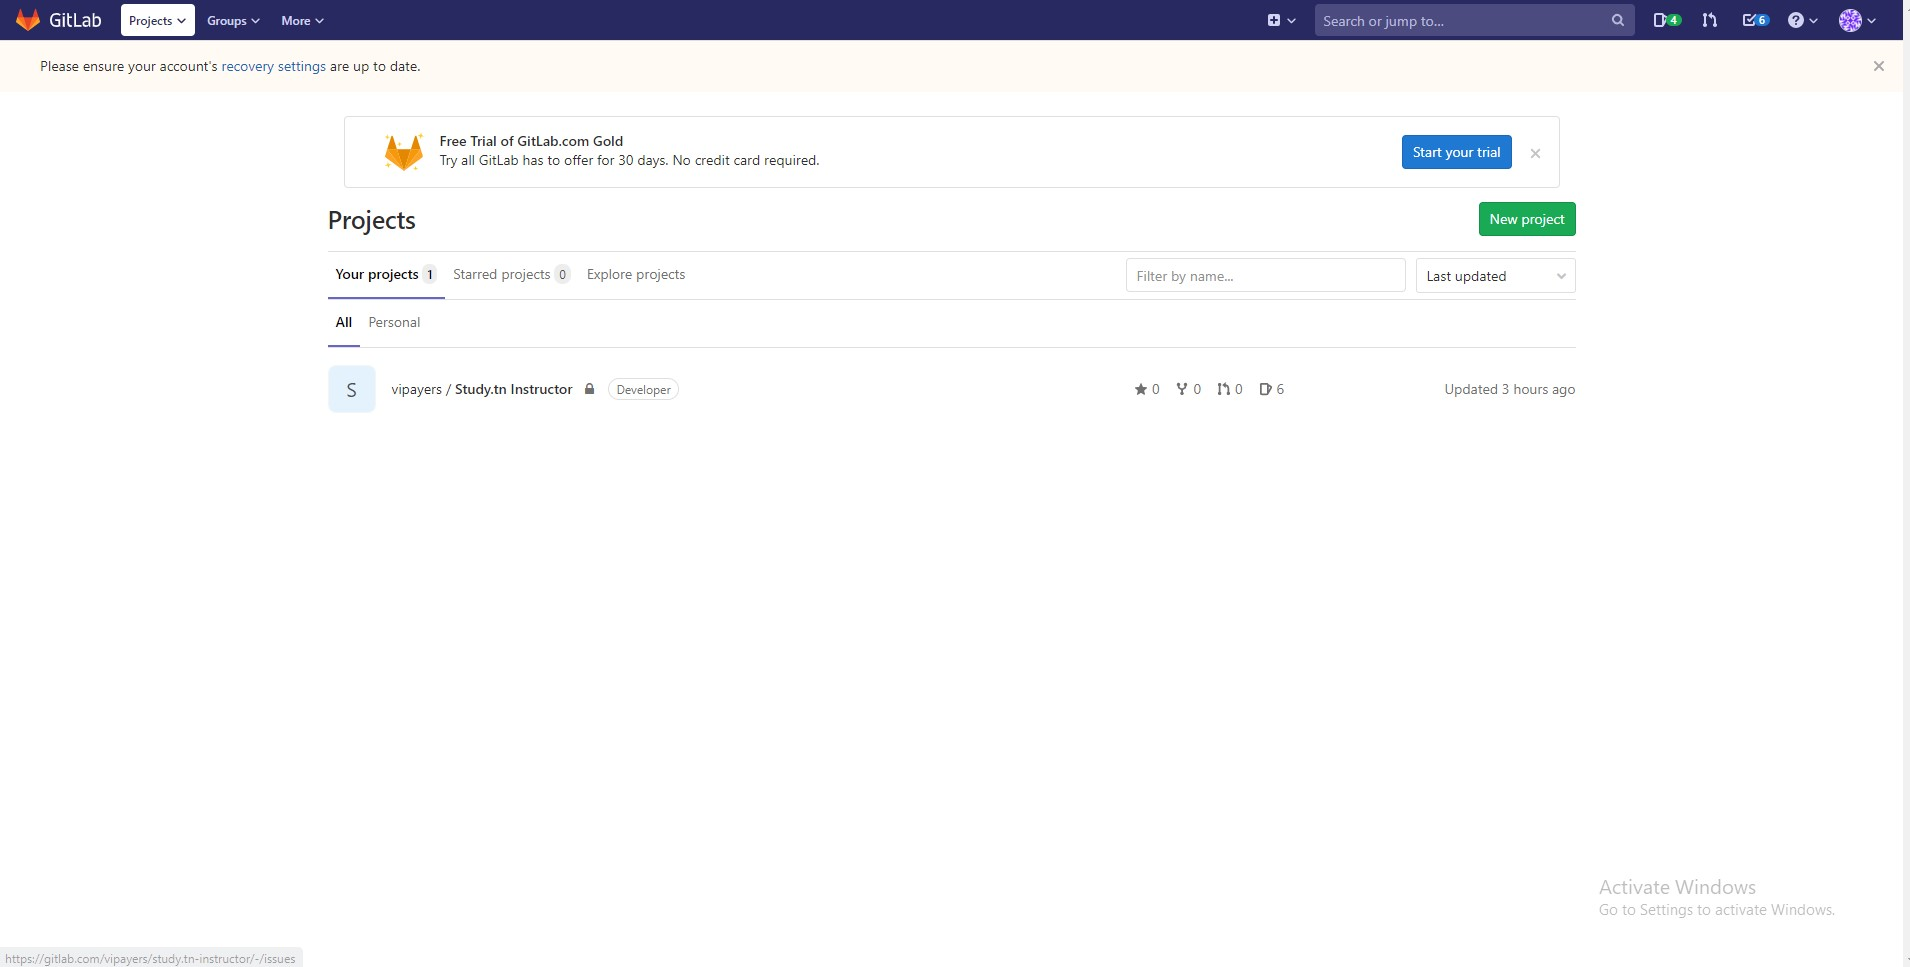
\includegraphics[width=150mm]{gitlab_interface.jpg}
    \caption{Gitlab interface}
    \label{fig:gitlab_interface}
\end{figure}

\vfill
\clearpage

\hfill \break
\hfill \break
\textbf{Slack \cite{cite6} :} Slack is a collaboration hub that can replace email to help you and your team work together seamlessly. It’s designed to support the way people naturally work together, so you can collaborate with people online as efficiently as you do face-to-face.

\begin{figure}[!ht]
    \centering
    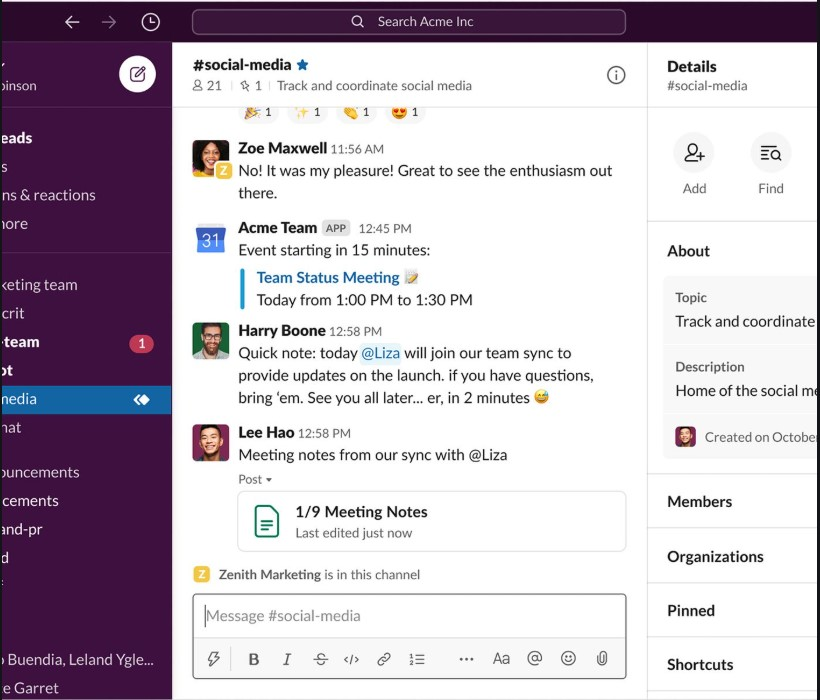
\includegraphics[width=150mm]{slack_interface.jpg}
    \caption{Slack interface}
    \label{fig:slack_interface}
\end{figure}


\section{Application architecture}

\vfill
\clearpage

\begin{figure}[!ht]
    \centering
    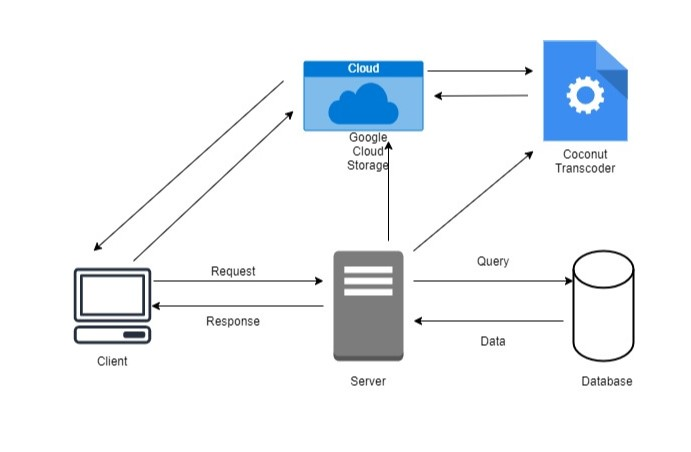
\includegraphics[width=150mm]{project_architecture.jpg}
    \caption{Application architecture}
    \label{fig:slack_interface}
\end{figure}



\section*{Conclusion}
In this chapter, we coved the application architecture, the hardware and software environment used in the project.

\addcontentsline{toc}{section}{Conclusion}
\chapter{SPRINT ONE - Manage courses}
\minitoc
\newpage
\section*{Introduction}
\addcontentsline{toc}{section}{Introduction}
In this sprint, we will be developing the authentication system and let the instructors manage their courses.
\section{Sprint backlog}
%%%%%table
\begin{table}[H]
\centering
\caption{Product backlog}
\begin{tabular}{|p{1cm}|p{3cm}|p{6cm}|p{2cm}|}
\hline
\rowcolor{brown!18}\textbf{\large{ID}} & \textbf{\large{As a}} & \textbf{\large{I want to be able to}} & \textbf{\large{Priority}} \\
\hline
1& Instructor  & Access the instructor space & High\\\hline
2& Instructor & Add courses  & High\\\hline
3& Instructor & Delete my courses  & High\\\hline
4& Instructor & Edit my courses  & High\\\hline

\end{tabular}
\end{table}
%%%%%table
\section{Requirement analysis}
\subsection{Use case diagram}

\begin{figure}[!ht]
\centering
     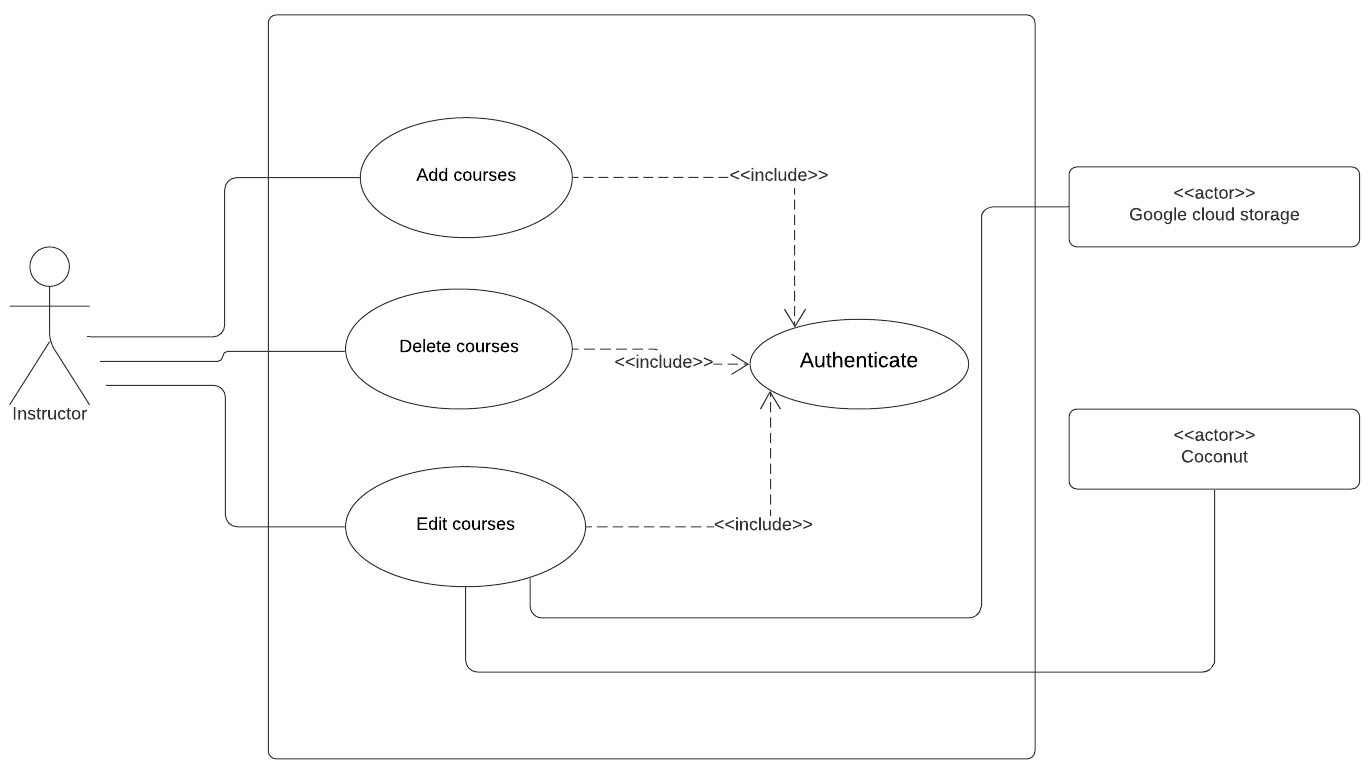
\includegraphics[width=150mm]{sprint1usecase.png}
    \caption{Sprint 1 use case diagram}
    \label{fig:sprint1usecase}
\end{figure}

\subsection{Modeling}

%%%%%table
\begin{table}[H]
\centering
\caption{add courses textual description}
\begin{tabular}{|p{4cm}|p{10cm}|}
\hline
\textbf{\large{Use case name}} & Add courses \\\hline
\textbf{\large{Actors}} & Instructor \\\hline
\textbf{\large{Preconditions}} & User logged in \\\hline
\textbf{\large{Postconditions}} & Course created  \\\hline
\textbf{\large{Normal flow}} & 
\begin{itemize}
  \item The instructor visits the instructor space.
  \item The instructor clicks the courses tab.
  \item The instructor clicks the add a course button.
\end{itemize}
\\\hline

\end{tabular}
\end{table}
%%%%%table

\begin{figure}[!ht]
    \centering
    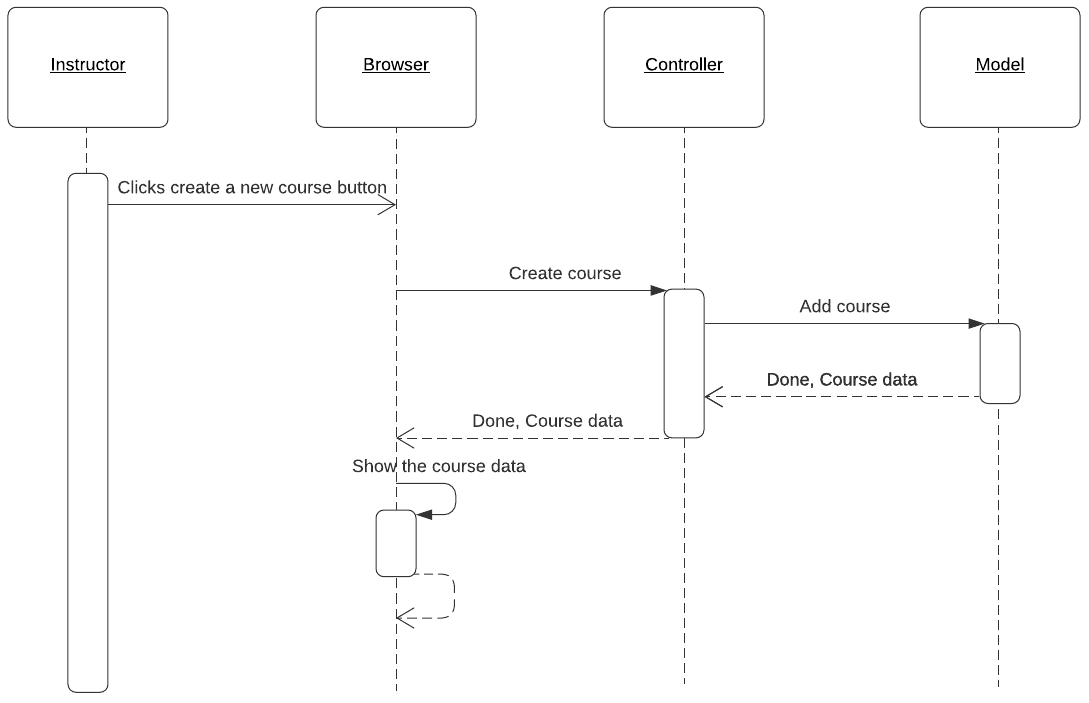
\includegraphics[width=142mm]{seq_create_course.png}
    \caption{Sequence diagram of creating a course}
    \label{fig:seq_create_course}
\end{figure}


%%%%%table
\begin{table}[H]
\centering
\caption{delete courses textual description}
\begin{tabular}{|p{4cm}|p{10cm}|}
\hline
\textbf{\large{Use case name}} & Delete courses \\\hline
\textbf{\large{Actors}} & Instructor \\\hline
\textbf{\large{Preconditions}} & User logged in \\\hline
\textbf{\large{Postconditions}} & Course created  \\\hline
\textbf{\large{Normal flow}} & 
\begin{itemize}
  \item The instructor visits the instructor space.
  \item The instructor clicks the courses tab.
  \item The instructor clicks on the course he wants to delete.
  \item The instructor use the delete button.
\end{itemize}
\\\hline

\end{tabular}
\end{table}
%%%%%table

\begin{figure}[!ht]
    \centering
    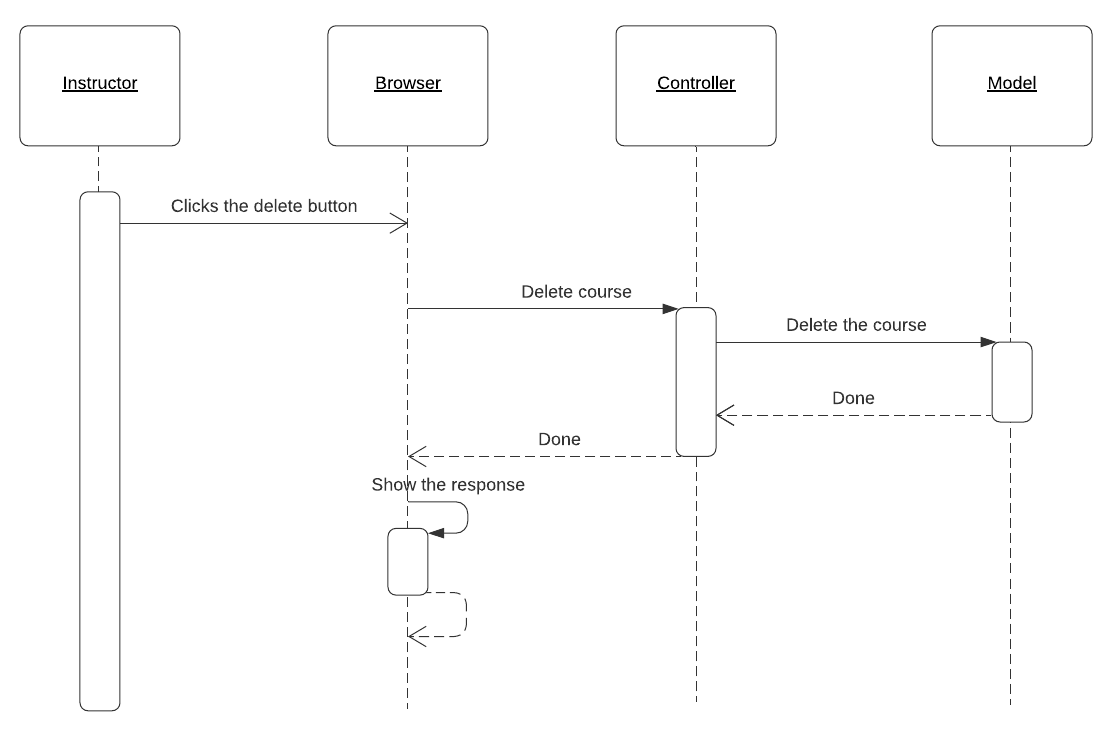
\includegraphics[width=150mm]{seq_delete_course.png}
    \caption{Sequence diagram of deleting a course}
    \label{fig:seq_delete_course}
\end{figure}

\newpage
\vfill

%%%%%table
\begin{table}[H]
\centering
\caption{edit courses textual description}
\begin{tabular}{|p{4cm}|p{10cm}|}
\hline
\textbf{\large{Use case name}} & Delete courses \\\hline
\textbf{\large{Actors}} & Instructor \\\hline
\textbf{\large{Preconditions}} & User logged in \\\hline
\textbf{\large{Postconditions}} & Course edited  \\\hline
\textbf{\large{Normal flow}} & 
\begin{itemize}
  \item The instructor visits the instructor space.
  \item The instructor clicks the courses tab.
  \item The instructor clicks on the course he wants to edit.
  \item The instructor type the meta data of the course.
  \item The instructor save the changes by using the save button.
\end{itemize}
\\\hline

\end{tabular}
\end{table}
%%%%%table

\begin{figure}[!ht]
    \centering
    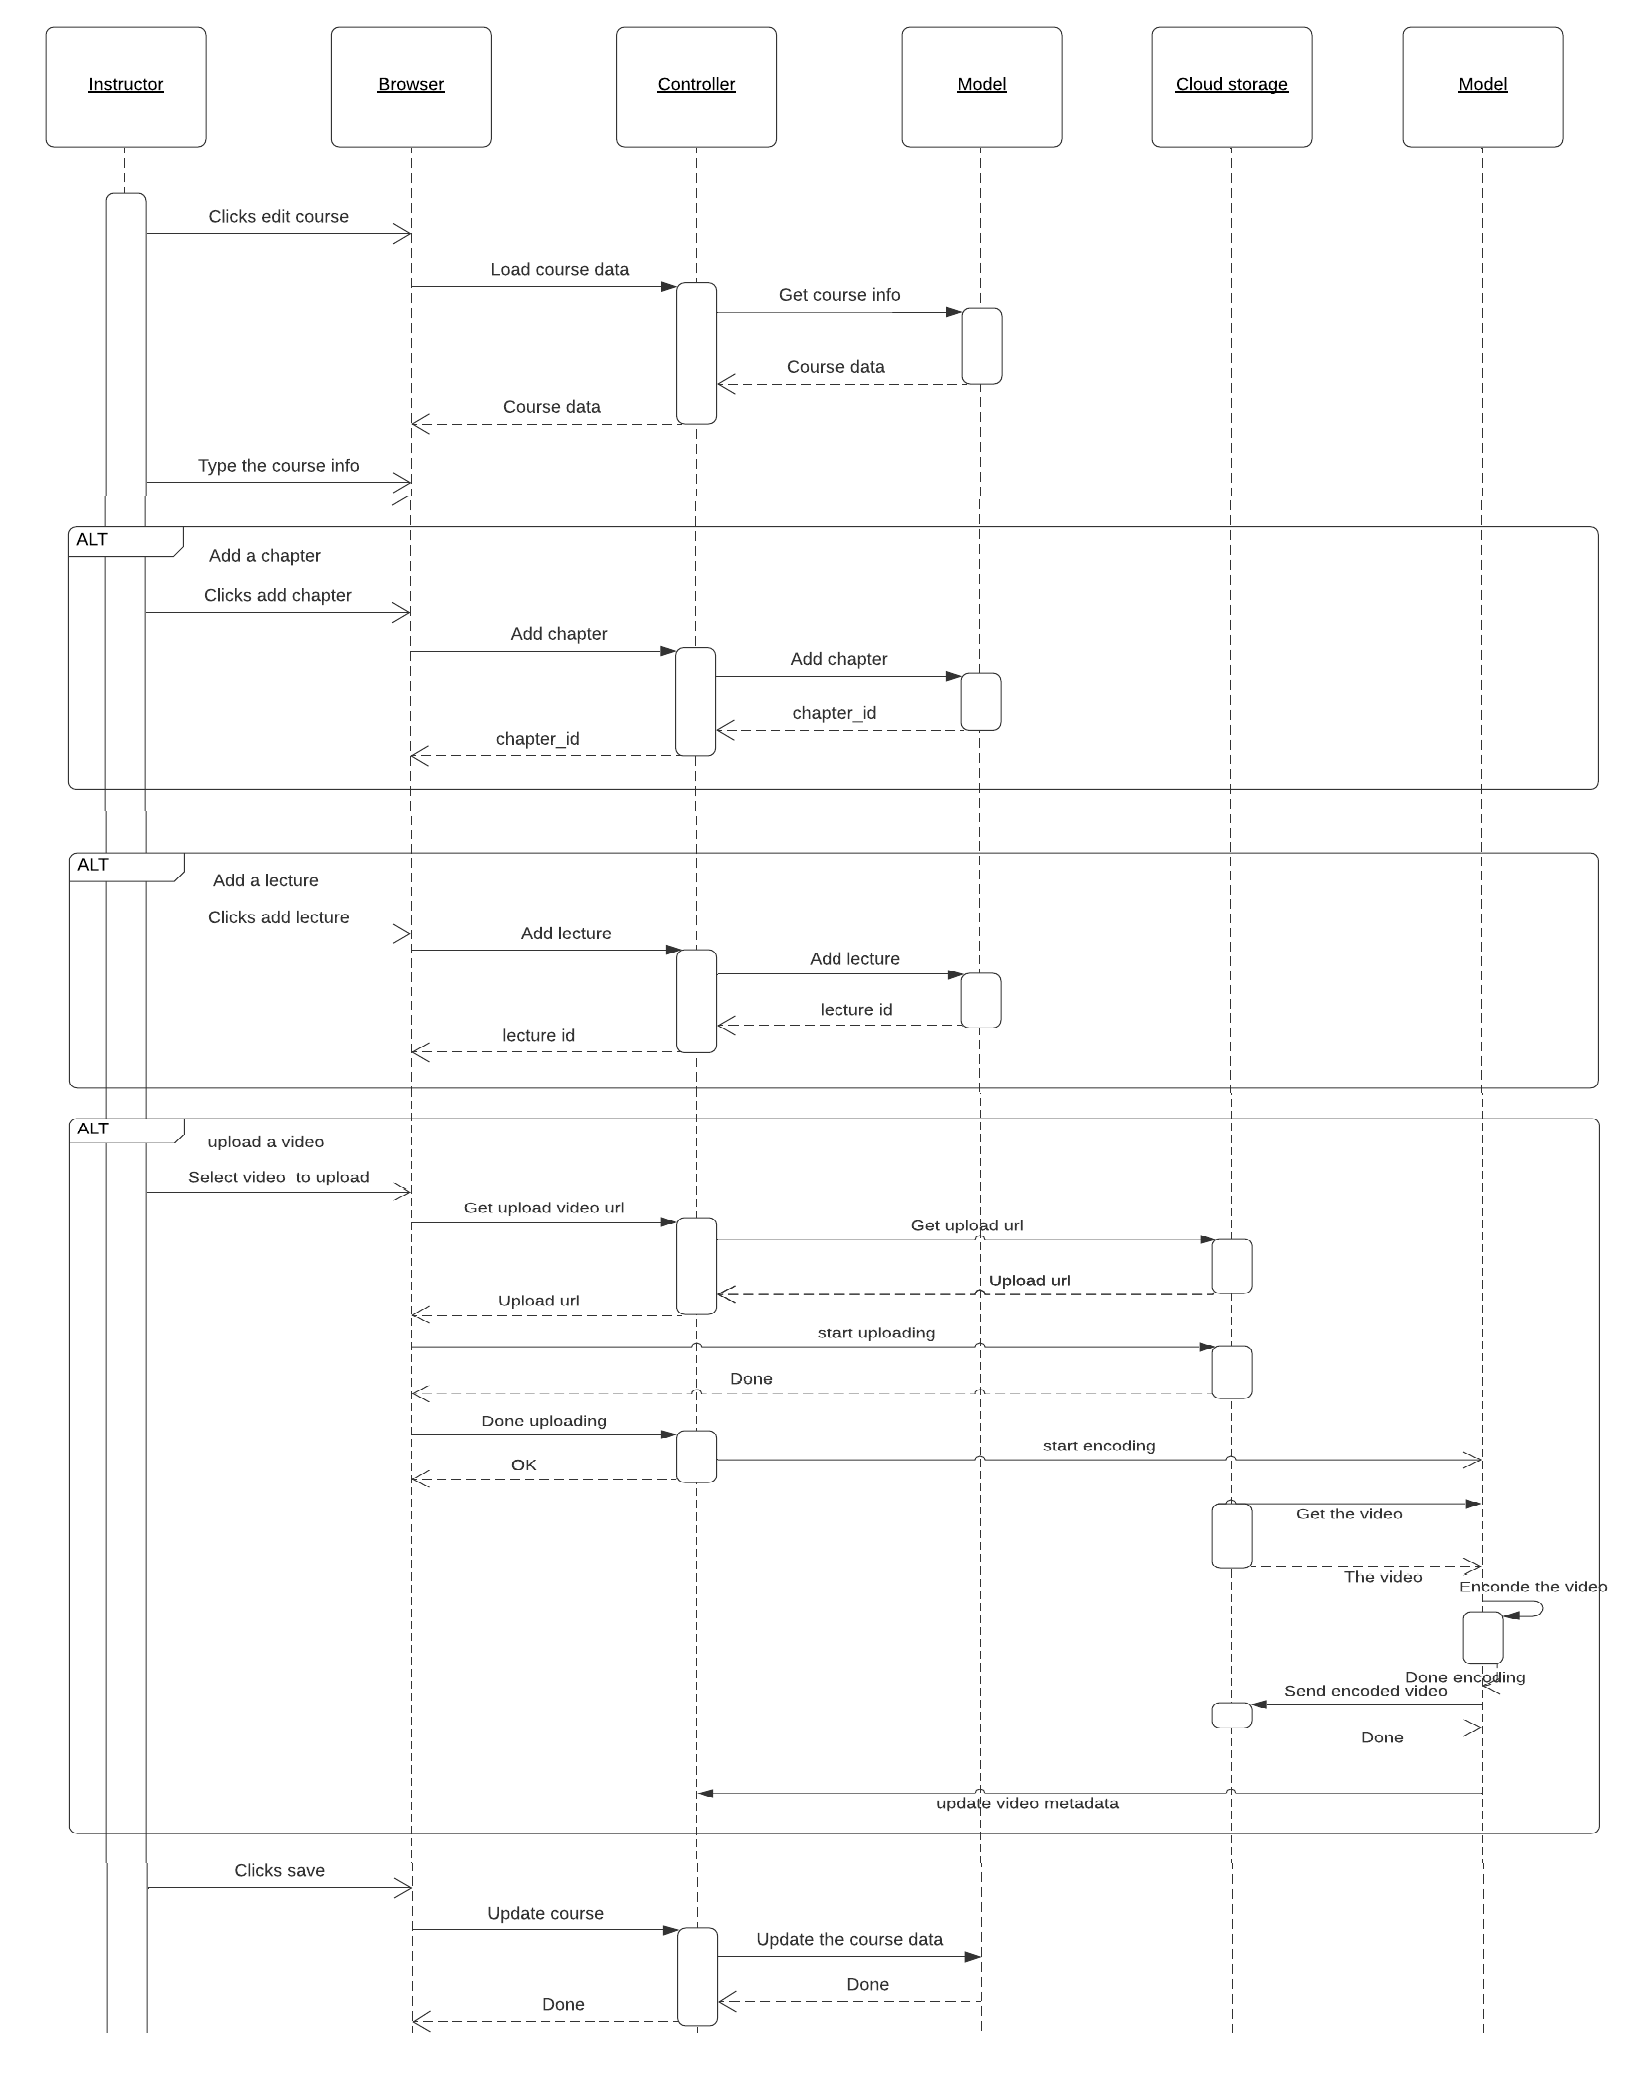
\includegraphics[width=170mm,height=200mm]{seq_edit_course.png}
    \caption{Sequence diagram of editing a course}
    \label{fig:seq_edit_course}
\end{figure}

\vfill
\clearpage

\section{Implementation}

\subsection{Access the instructor space}
As study.tn website already has its own authentication system, the instructor only needs to log in to study.tn then visit the instructor space. Since study.tn and the instructor dashboard are both separate apps, we need to let our app know who's the logged in user in study.tn. Once the instructor tries to visit the dashboard from study.tn we send the authentication token to our dashboard in the url, we get that token, save it in the local storage and then we know who's the user accessing the dashboard with that token.

\subsection{Add a course}
When clicking on the add course button, we make a request to the server to add a new course to the database and as a response we get the created record data (course id, course name...) which is then added to the redux store state to update and re-render the courses.

\subsection{Delete a course}
When clicking on the delete course button, we send a request with the course id to the server to remove the course from the database and show the result of the response to the user accordingly. If no one is enrolled in that course we should recieve a success and remove the course from the redux store to re-render the courses list. 

\begin{figure}[!ht]
    \centering
    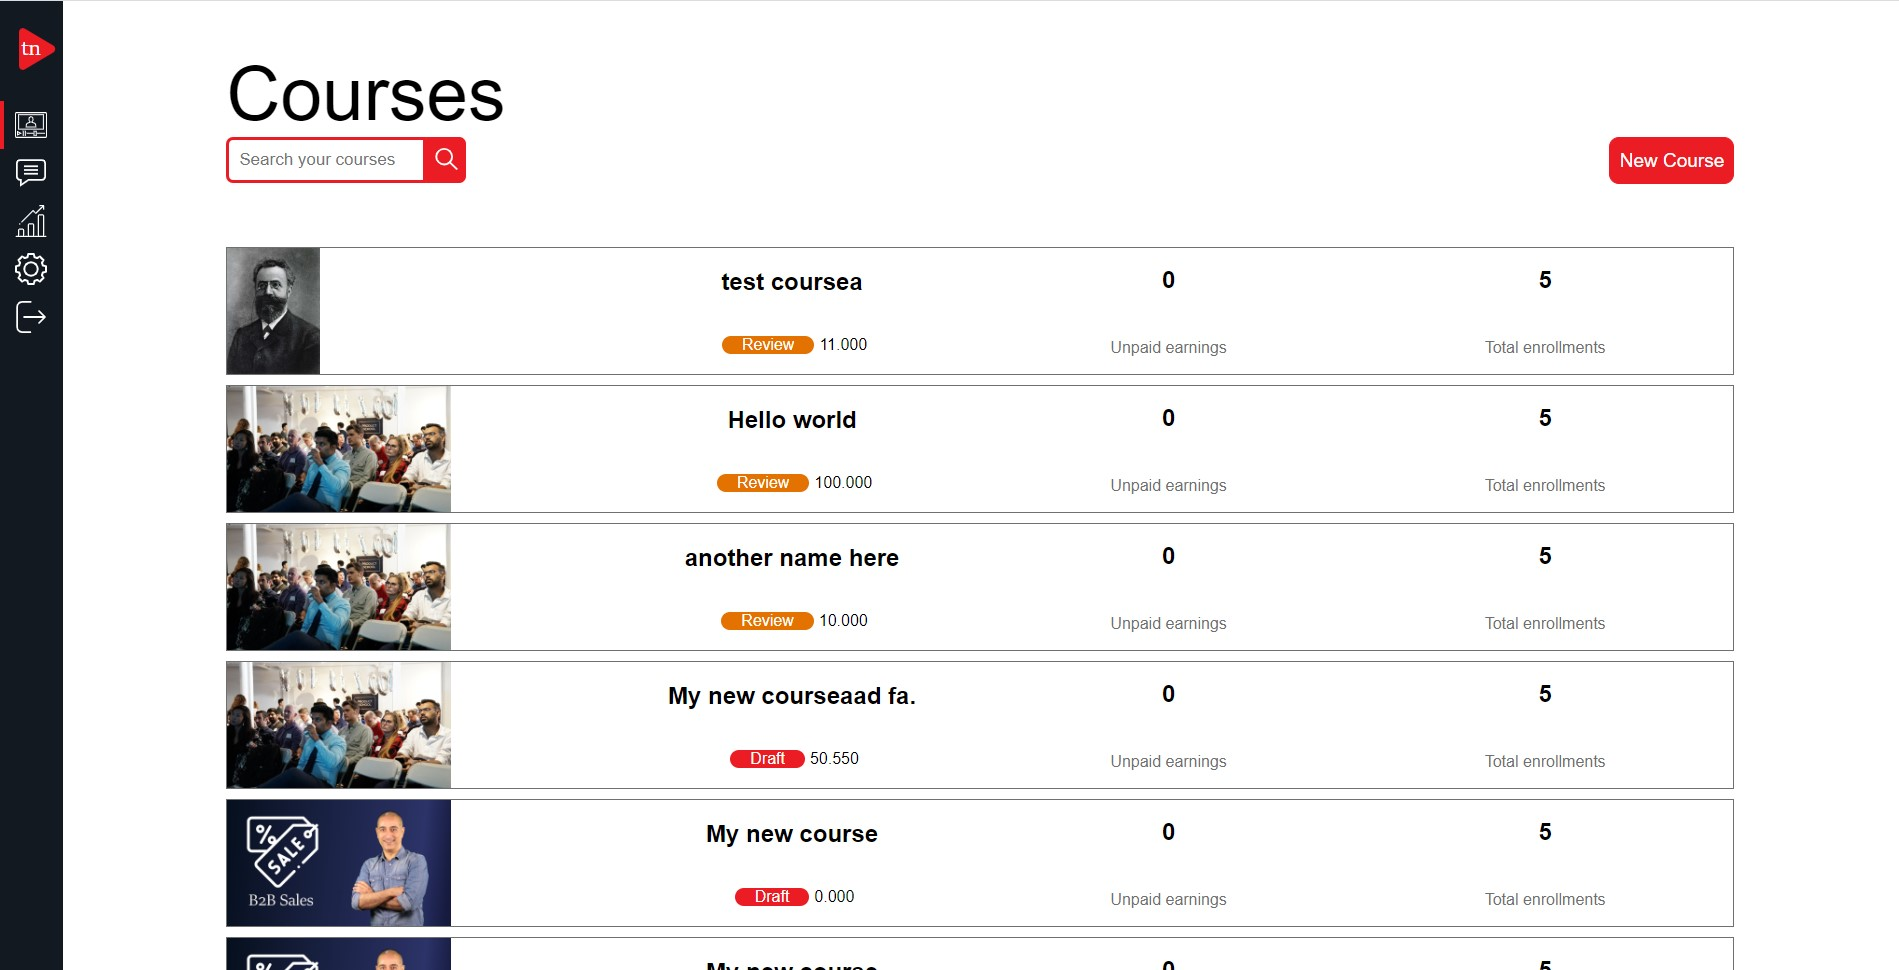
\includegraphics[width=150mm]{courses_tab2.jpg}
    \caption{Courses tab interface}
    \label{fig:courses_tab2}
\end{figure}

\subsection{Edit course}
Clicking on the course in the courses list will bring up a page where the instructor can edit the course and he must fill in the meta data of the course. The page consists of multiple forms each having it's own redux reducer and each form will load it's data individually.

\subsubsection{Target student form}
The instructor writes what are the requirements and prerequisites that students need to have to understand the course in the input field and click the plus button to add it, which will fire a post request to the server sending the text in the input field. When the request is running we show a loader to the user to let him know that something is happening in the background and he needs to wait. After a successful request we update the form state to add the requirement and re-render the form.

\hfill \break
\hfill \break
The instructor can change the order of the requirements list using drag and drop. We implemented it with the help of react-sort-list library which sort the list in the front end, once it's done we make a post request to the server with the requirements new order in the body.
\hfill \break
\hfill \break
We can also delete a requirement by clicking the bin icon and let the server know that we want to delete the element.
\hfill \break
\hfill \break
The process is the same for what will the student learn list.

\vfill
\clearpage

\begin{figure}[!ht]
    \centering
    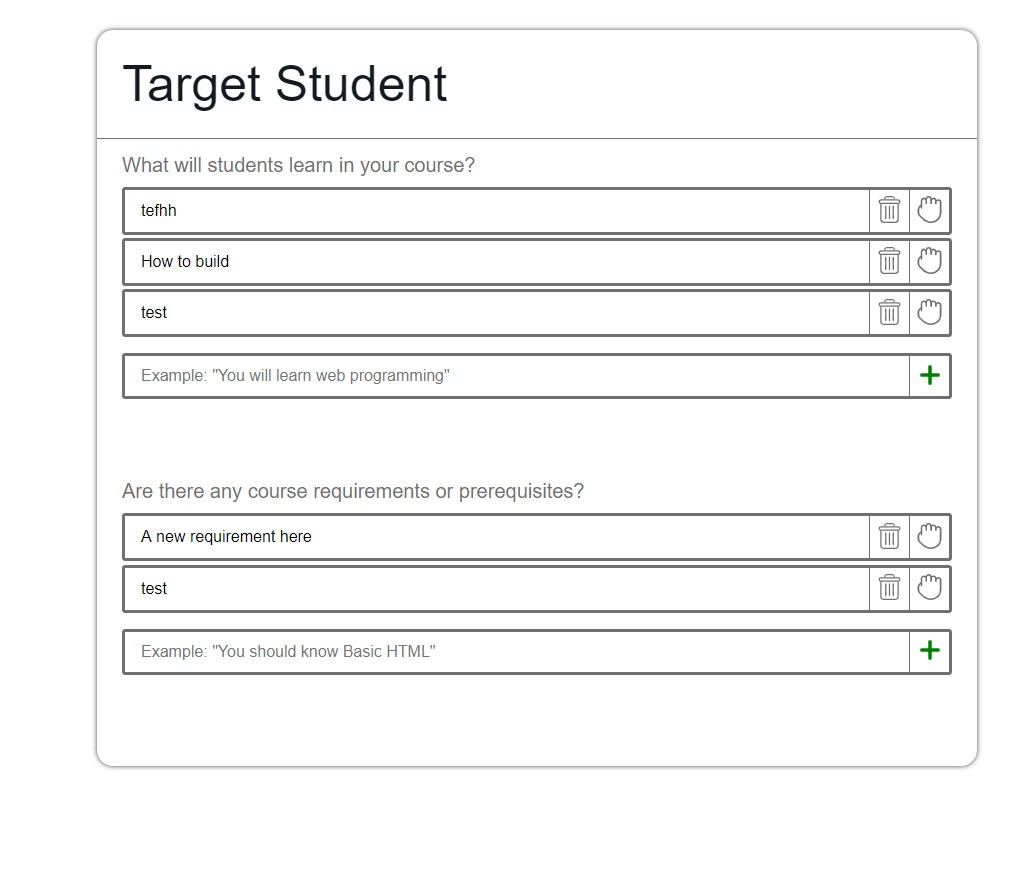
\includegraphics[width=150mm]{target_student_form.jpg}
    \caption{Target student form interface}
    \label{fig:target_student_form}
\end{figure}


\subsubsection{Curriculum form}
A course is composed of chapters, each chapter could have one or more lectures. A lecture is simply a video, but it could have a file as well.
\hfill \break
\hfill \break
We can add a new chapter by clicking add a new chapter button, the browser will make a request to the server and in return we get the created chapter data which we can use to update the redux state and show the new chapter to the user. We can delete a chapter by clicking the bin icon or edit it by clicking the bin icon, let the server know then update the interface. We can also sort the chapter in the same way we did in the target form with the help of react-sort-list library.
\hfill \break
\hfill \break
The same actions performed on chapters can be performed on lectures and they share the same implementation. However, We can upload a video to a lecture by selecting a video, the browser will then make a request to the server to get an upload url and the video id associated to the video that we are about to upload then the upload will start. As the upload process can take time, we show the user a progress bar with a percentage on it. Once it's done we make another request to let the server know that the video has been uploaded successfully and associate the video id with the lecture. Since the video is transcoding and we don't know when this process will end, we refresh the lecture with a random timer between 20 second and 40 seconds to check if the video is ready and show it to the user. The reason behind picking a random timer is to minimize the load on the server so it's less likely that many users will make a request at the same time. The process of uploading a file is as the same as the video except the transcoding phase.

\begin{figure}[!ht]
    \centering
    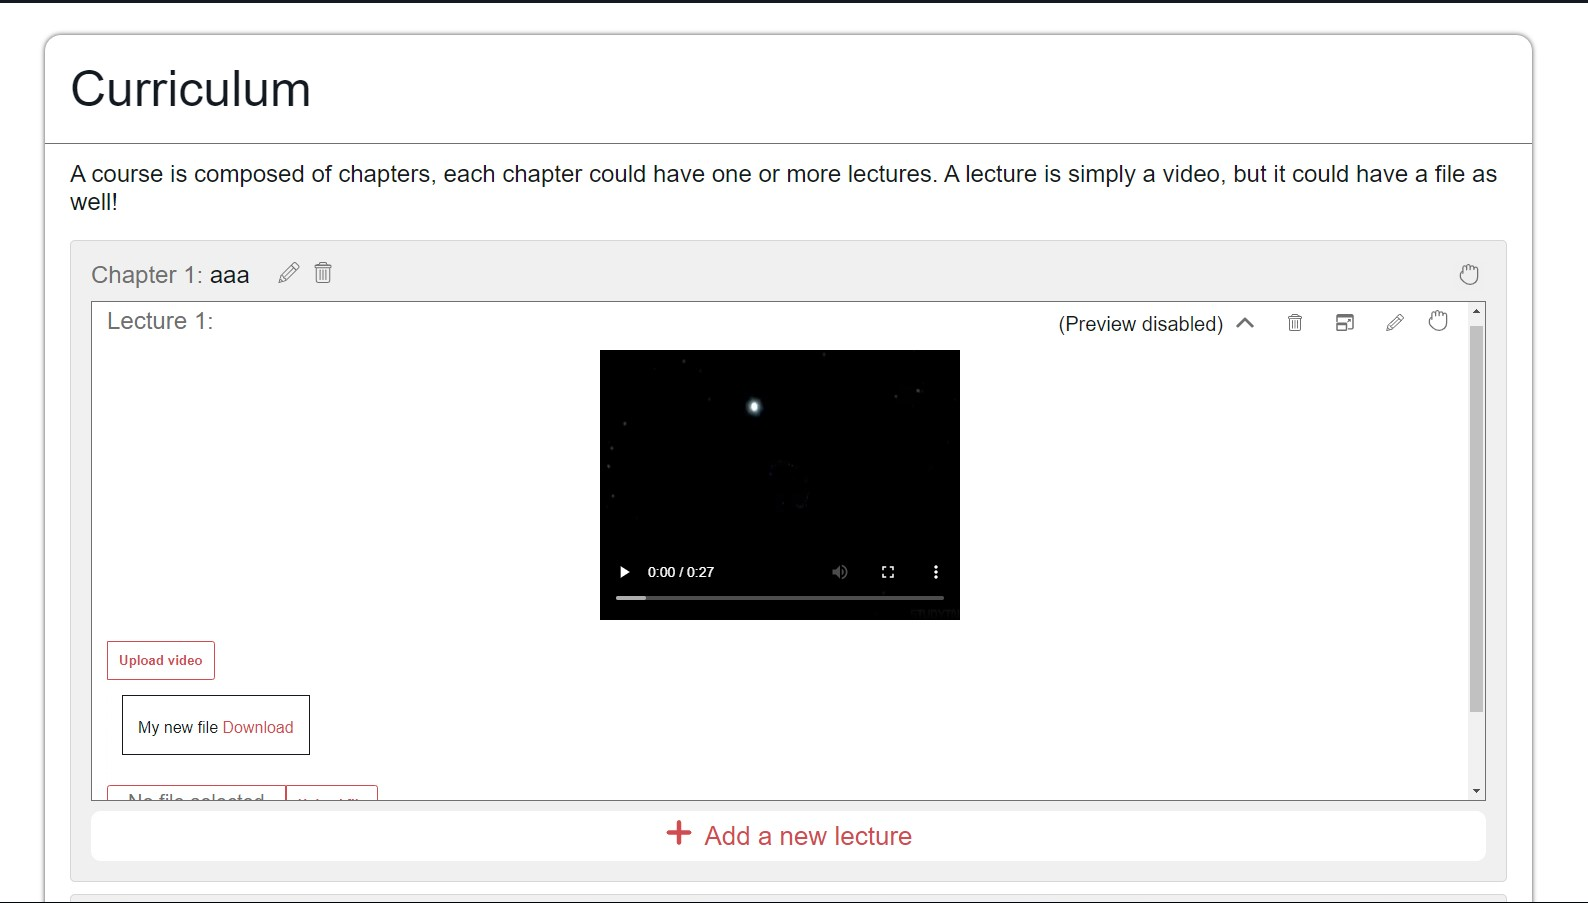
\includegraphics[width=150mm]{curriculum_form.jpg}
    \caption{Curriculum form interface}
    \label{fig:curriculum_form}
\end{figure}


\subsubsection{Landing page form}
In the landing page form, the user types the course info (title, subtitle, description...) and clicks the save button to update the course informations.

\vfill
\clearpage

\begin{figure}[!ht]
    \centering
    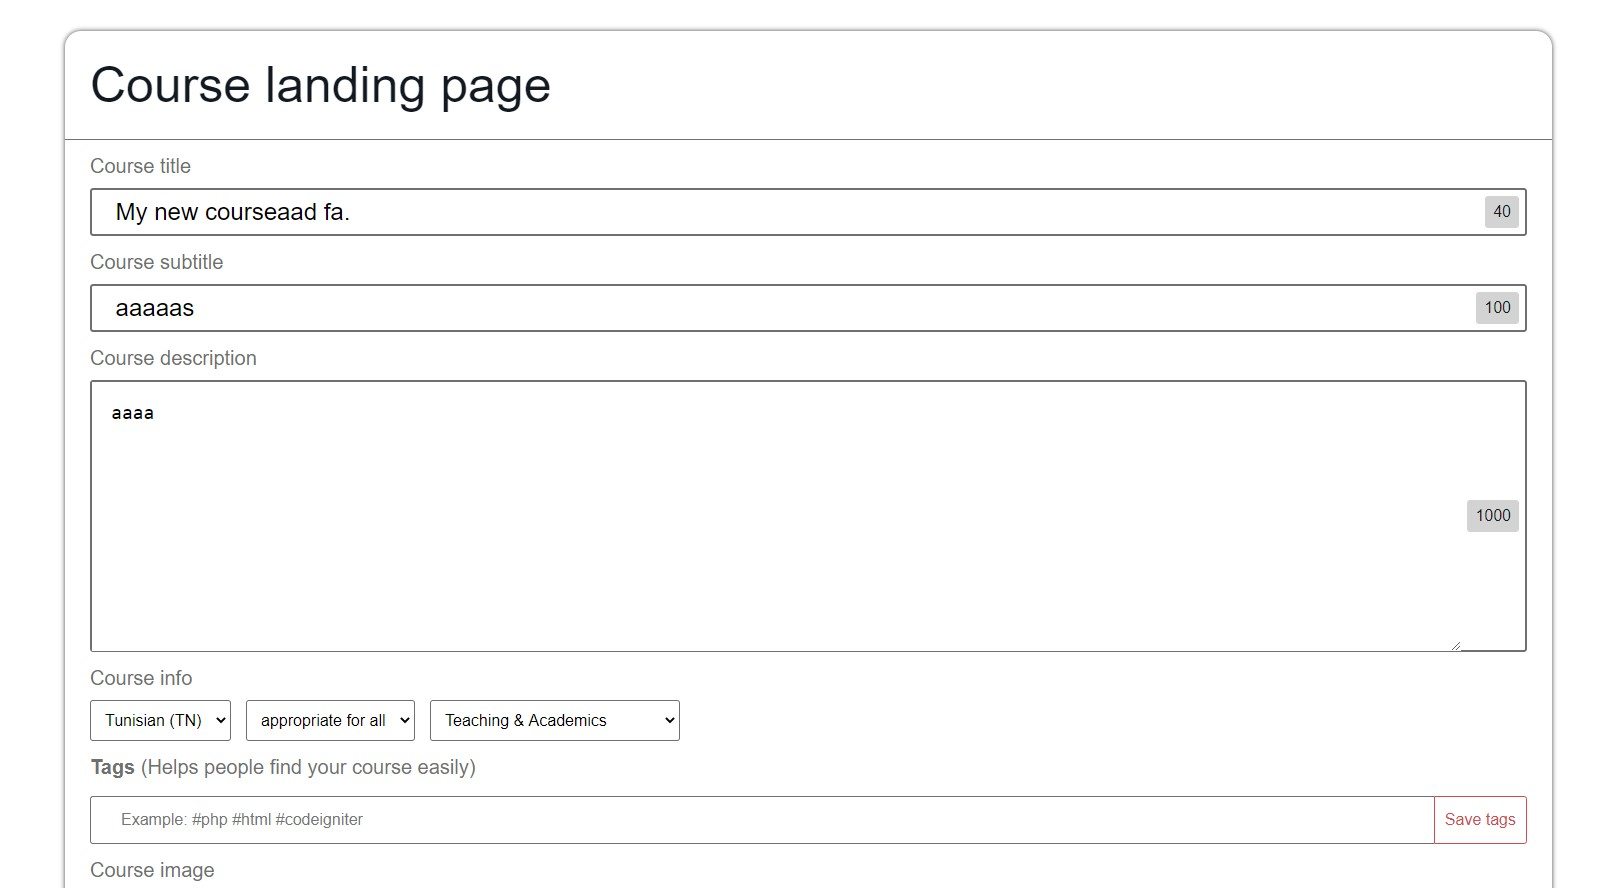
\includegraphics[width=150mm]{landing_page_form.jpg}
    \caption{Landing page form interface}
    \label{fig:landing_page_form}
\end{figure}


\subsubsection{Pircing form}
The instructor puts the price he wants in TND then clicks the save button to make a request to the server and update the price.

\begin{figure}[!ht]
    \centering
    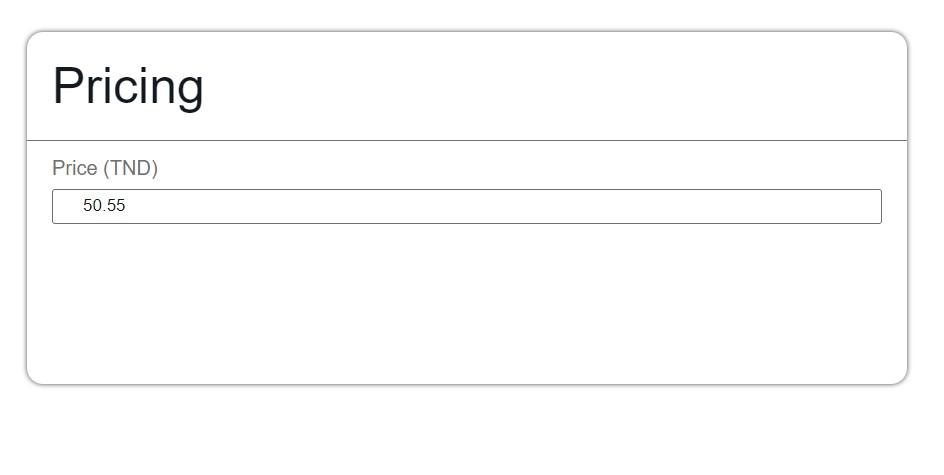
\includegraphics[width=150mm]{price_form.jpg}
    \caption{Pircing form interface}
    \label{fig:price_form}
\end{figure}

\vfill
\clearpage

\section*{Conclusion}
In this chapter, we coved how the instructor can manage his courses and access the dashboard.

\addcontentsline{toc}{section}{Conclusion}
\chapter{SPRINT TWO - Communication and sales}
\minitoc
\newpage
\section*{Introduction}
\addcontentsline{toc}{section}{Introduction}
In this sprint, we will be developing the part where the instructor will communicate with the students and manage the sales.
\section{Sprint backlog}
%%%%%table
\begin{table}[H]
\centering
\caption{Product backlog}
\begin{tabular}{|p{1cm}|p{3cm}|p{6cm}|p{2cm}|}
\hline
\rowcolor{brown!18}\textbf{\large{ID}} & \textbf{\large{As a}} & \textbf{\large{I want to be able to}} & \textbf{\large{Priority}} \\
\hline
5& Instructor & Send messages to my students & High\\\hline
6& Instructor & Recieve messages from my students  & High\\\hline
7& Instructor  & See my course sales & Normal \\\hline
\end{tabular}
\end{table}
%%%%%table
\section{Requirement analysis}
\subsection{Use case diagram}

\begin{figure}[!ht]
    \centering
    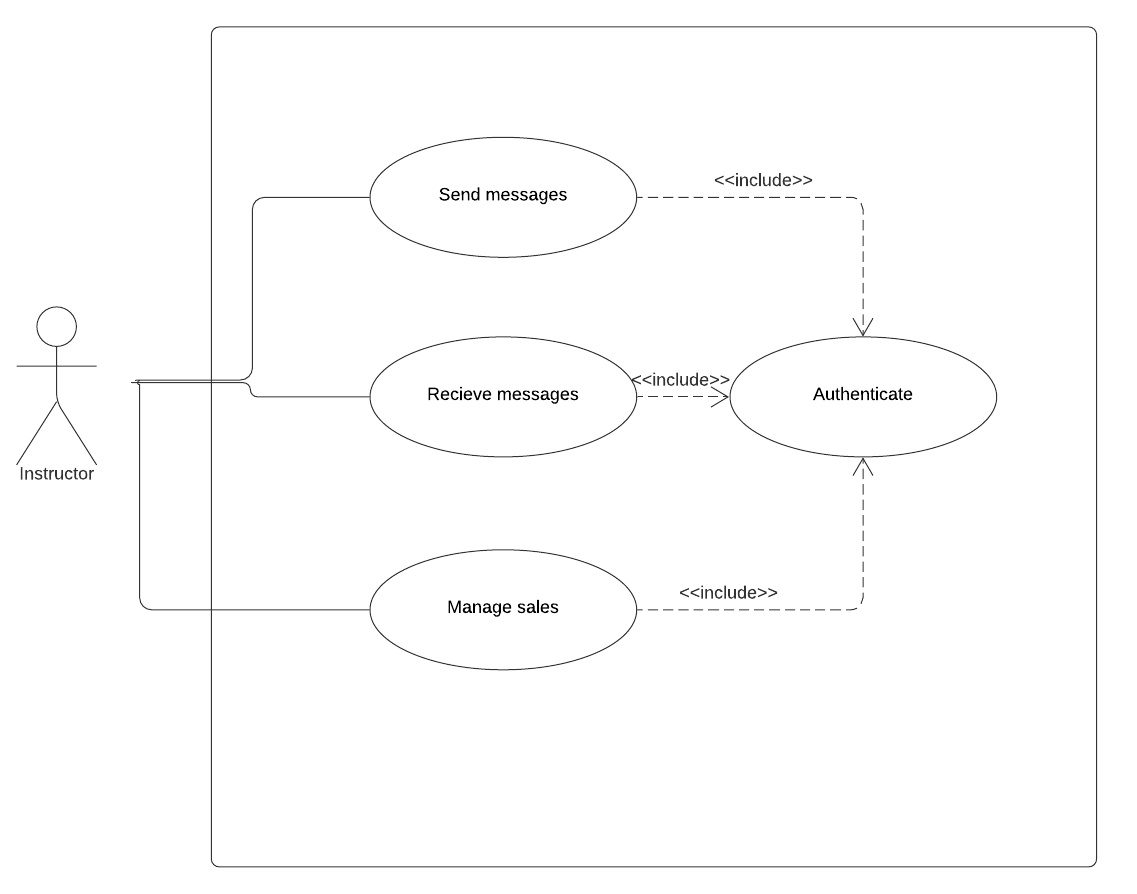
\includegraphics[width=120mm]{sprint2usecase.png}
    \caption{Sprint 2 use case diagram}
    \label{fig:sprint2usecase}
\end{figure}




\subsection{Modeling}

%%%%%table
\begin{table}[H]
\centering
\caption{send messages textual description}
\begin{tabular}{|p{4cm}|p{10cm}|}
\hline
\textbf{\large{Use case name}} & Send messages \\\hline
\textbf{\large{Actors}} & Instructor \\\hline
\textbf{\large{Preconditions}} & User logged in \\\hline
\textbf{\large{Postconditions}} & Message sent  \\\hline
\textbf{\large{Normal flow}} & 
\begin{itemize}
  \item The instructor visits the instructor space.
  \item The instructor clicks the communication tab.
  \item The instructor opens the conversation.
  \item The instructor type the message and clicks send.
\end{itemize}
\\\hline

\end{tabular}
\end{table}
%%%%%table

\begin{figure}[!ht]
    \centering
    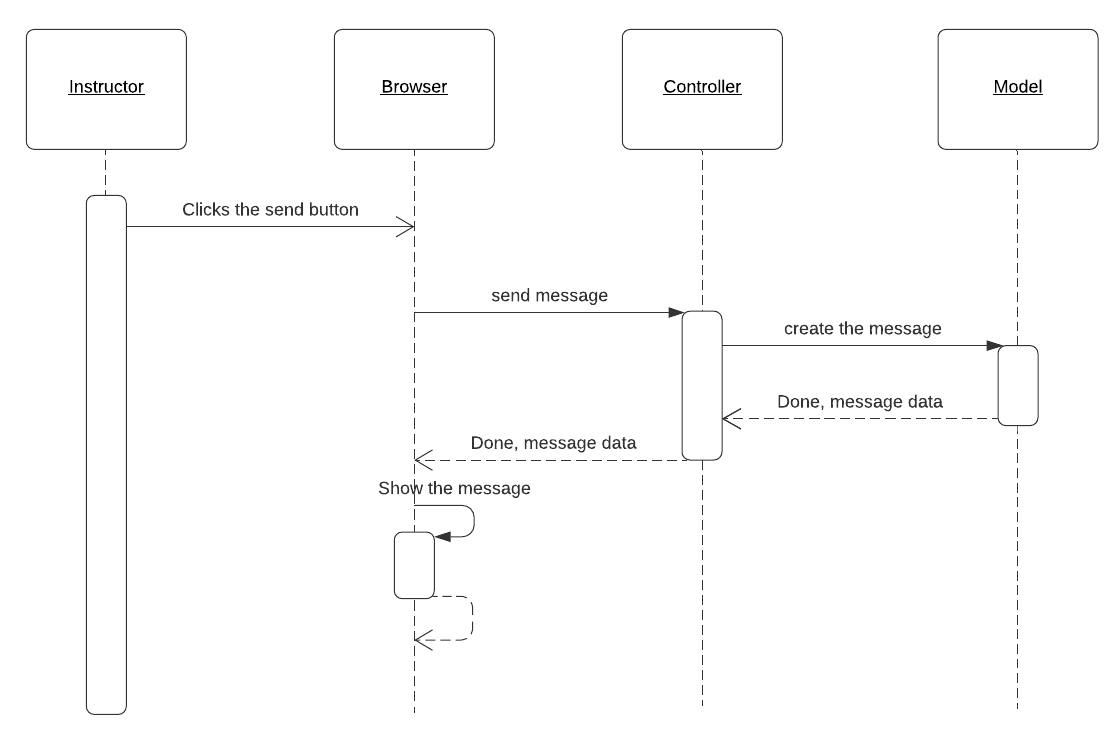
\includegraphics[width=142mm]{seq_send_message.png}
    \caption{Sequence diagram of sending a message}
    \label{fig:seq_send_message}
\end{figure}

%%%%%table
\begin{table}[H]
\centering
\caption{recieve messages textual description}
\begin{tabular}{|p{4cm}|p{10cm}|}
\hline
\textbf{\large{Use case name}} & Recieve messages \\\hline
\textbf{\large{Actors}} & Instructor \\\hline
\textbf{\large{Preconditions}} & User logged in \\\hline
\textbf{\large{Postconditions}} & Message recieved and seen \\\hline
\textbf{\large{Normal flow}} & 
\begin{itemize}
  \item The instructor visits the instructor space.
  \item The instructor clicks the communication tab.
  \item The instructor opens the conversation.
  \item The instructor type sees the messages recieved.
\end{itemize}
\\\hline

\end{tabular}
\end{table}
%%%%%table

\begin{figure}[!ht]
    \centering
    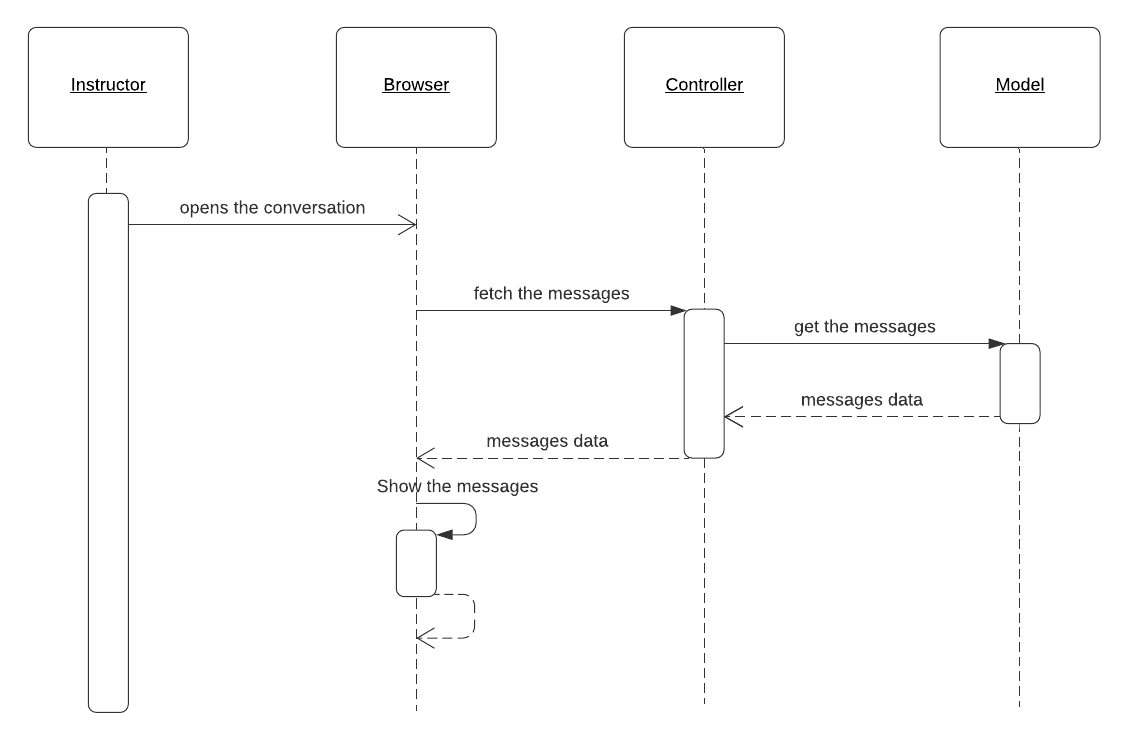
\includegraphics[width=150mm]{seq_recieve_message.png}
    \caption{Sequence diagram of recieving a message}
    \label{fig:seq_recieve_message}
\end{figure}

%%%%%table
\begin{table}[H]
\centering
\caption{manage sales textual description}
\begin{tabular}{|p{4cm}|p{10cm}|}
\hline
\textbf{\large{Use case name}} & Manage sales \\\hline
\textbf{\large{Actors}} & Instructor \\\hline
\textbf{\large{Preconditions}} & User logged in \\\hline
\textbf{\large{Postconditions}} & Sales managed  \\\hline
\textbf{\large{Normal flow}} & 
\begin{itemize}
  \item The instructor visits the instructor space.
  \item The instructor clicks the performance tab.
  \item The instructor sees statistics about their sales and earnings.
\end{itemize}
\\\hline

\end{tabular}
\end{table}
%%%%%table


\begin{figure}[!ht]
    \centering
    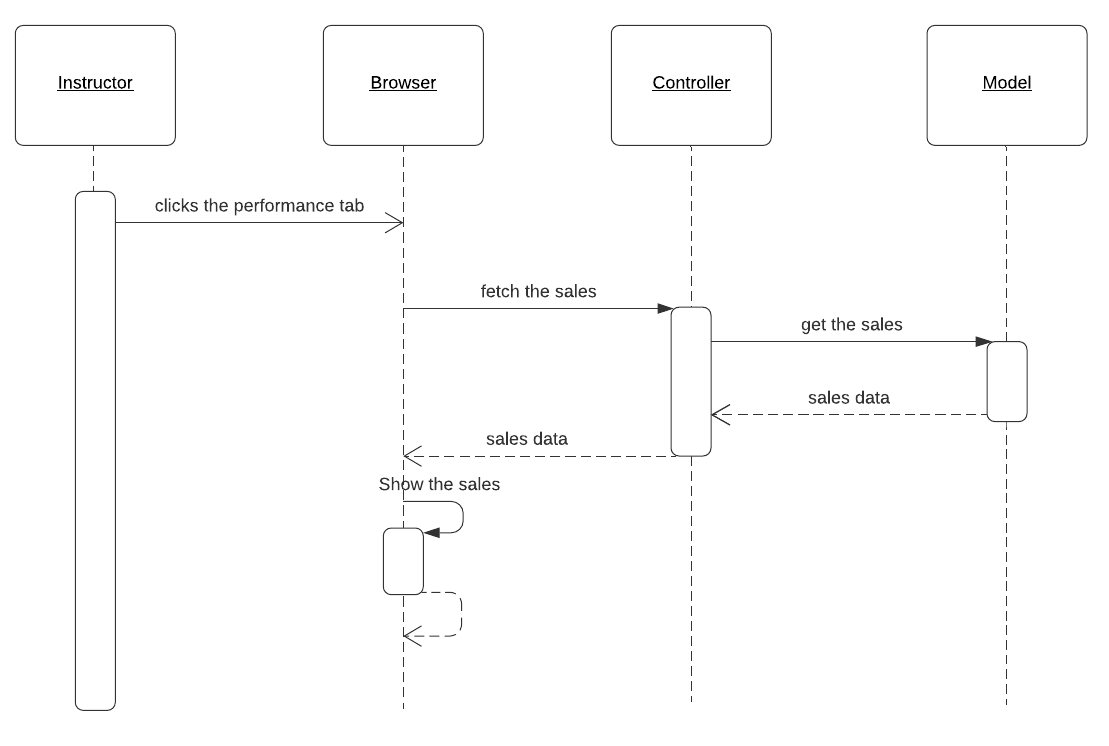
\includegraphics[width=150mm]{seq_sales.png}
    \caption{Sequence diagram of visitng sales}
    \label{fig:seq_sales}
\end{figure}


\section{Implementation}


\subsection{Sending a message}
When clicking on the send button, we send the message written to the server and in return we get the created record in the database. We add the result to the redux messages reducer to update the interface and show the sent message.

\subsection{Recieving messages}
Upon opening a conversation, the browser will make a request to the server to fetch the message of that conversation and show it to the user.
\hfill \break
Since we are not building a chat app, we avoided using realtime solutions like sockets to fetch messages without refreshing the page as it will cause more load on the server. So we chose to do long polling :  pick a random timer in a specific range and each time that timer expires we make a request to the server looking for new messages and show them to the user. 

\begin{figure}[!ht]
    \centering
    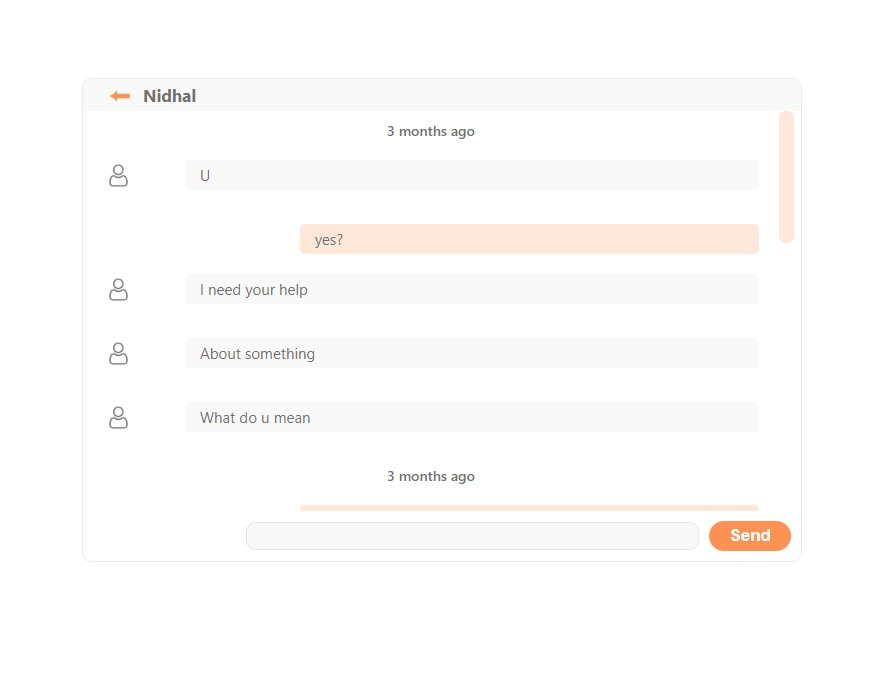
\includegraphics[width=150mm]{conversation2.jpg}
    \caption{Conversation interface}
    \label{fig:conversation2}
\end{figure}

\subsection{Manage Sales}
Clicking on the performance tab will bring up a page where the instructor see statistics about their sales and earnings. Upon visiting this page, the browser will make a request to the server to fetch all the necessary data and show them to the user.
\hfill \break
\hfill \break
We used react-chartjs-2 library to show the earnings of each month for the user in a graph. 
\hfill \break
\hfill \break
We also used react-data-table-component library to show the sales data in a table, this library helps us with sorting the data by a specific colum. The sorting happens in the server, so each time the user chose to sort by certain colum, we send a request to the server with the colum that we want to sort on, get the data and show it to the user accordingly. The library also helps us with the server side pagination, so that each time the user request a specific page we send a request to the server with the page number and fetch the data. 

\hfill \break
\hfill \break

\begin{figure}[!ht]
    \centering
    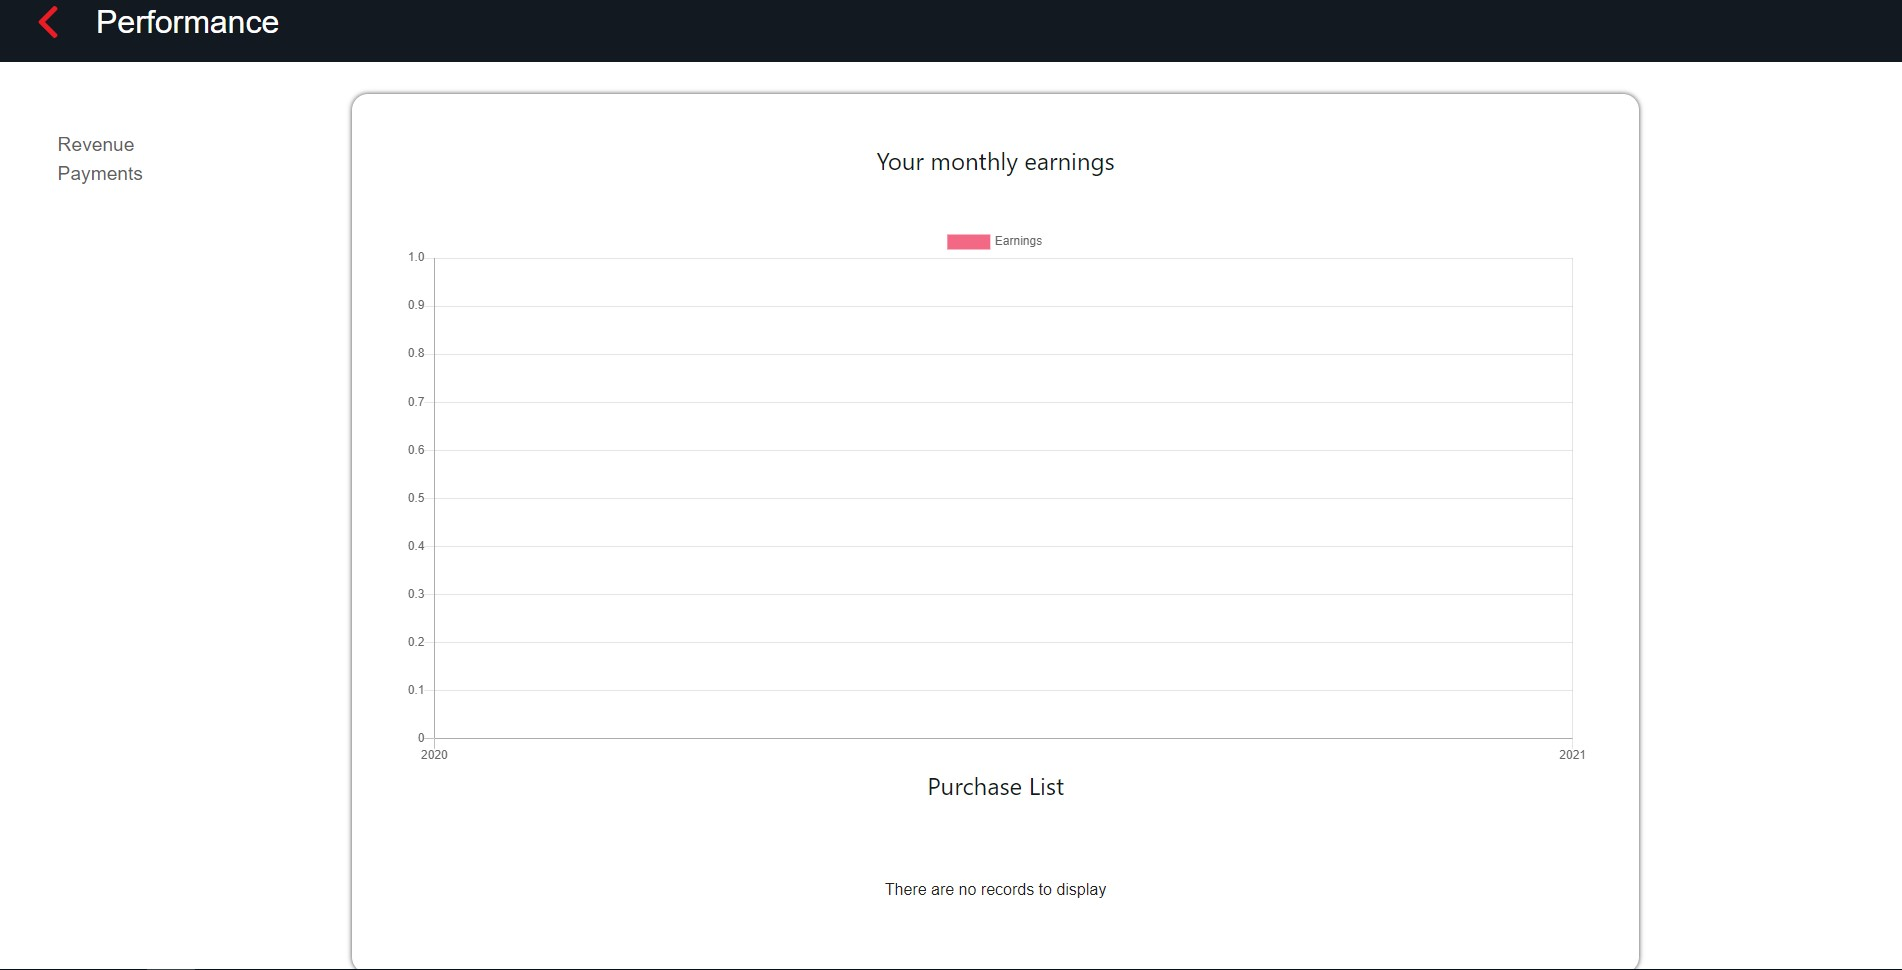
\includegraphics[width=150mm]{earnings.jpg}
    \caption{Sales page interface}
    \label{fig:earnings}
\end{figure}


\vfill
\clearpage

\section*{Conclusion}
In this chapter, we coved the communication part of the app and how the instructor can manage his sales.
\addcontentsline{toc}{section}{Conclusion}
\chapter{SPRINT THREE - Exam and apply to become an instructor}
\minitoc
\newpage
\section*{Introduction}
\addcontentsline{toc}{section}{Introduction}
In this sprint, we will take a look at how the instructor can create an exam and how a user can apply to become an instructor.
\section{Sprint backlog}
%%%%%table
\begin{table}[H]
\centering
\caption{Product backlog}
\begin{tabular}{|p{1cm}|p{3cm}|p{6cm}|p{2cm}|}
\hline
\rowcolor{brown!18}\textbf{\large{ID}} & \textbf{\large{As a}} & \textbf{\large{I want to be able to}} & \textbf{\large{Priority}} \\
\hline
8& Instructor & Create an exam & High\\\hline
9& User & Apply to become an instuctor  & Normal \\\hline
\end{tabular}
\end{table}
%%%%%table
\section{Requirement analysis}
\subsection{Use case diagram}

\begin{figure}[!ht]
    \centering
    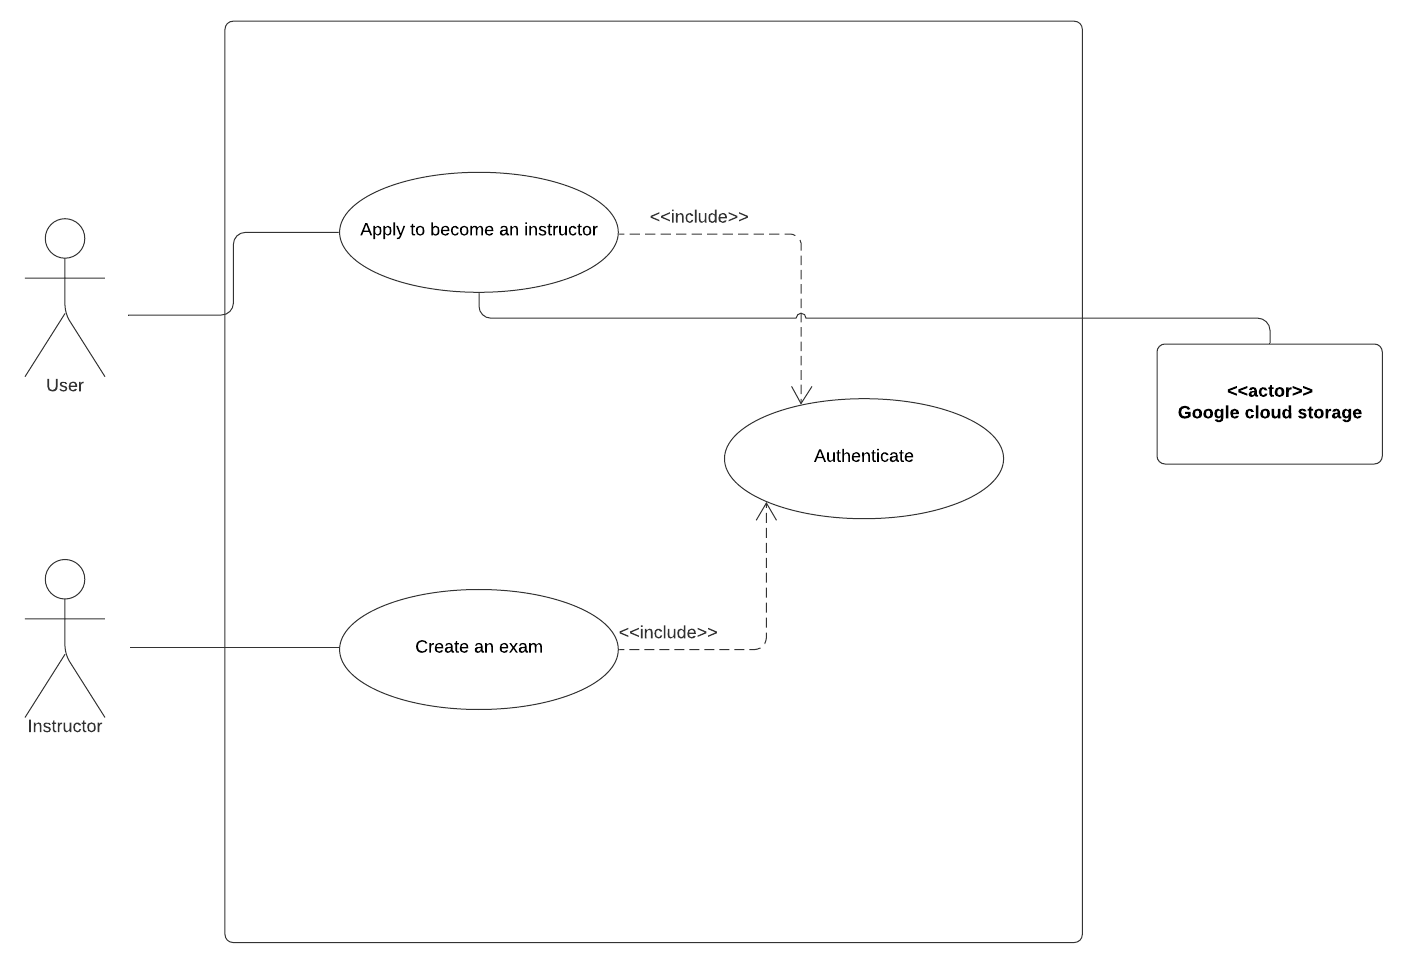
\includegraphics[width=130mm]{sprint3usecase.png}
    \caption{Sprint 3 use case diagram}
    \label{fig:sprint3usecase}
\end{figure}



\section{Modeling}

%%%%%table
\begin{table}[H]
\centering
\caption{create an exam textual description}
\begin{tabular}{|p{4cm}|p{10cm}|}
\hline
\textbf{\large{Use case name}} & Create an exam \\\hline
\textbf{\large{Actors}} & Instructor \\\hline
\textbf{\large{Preconditions}} & User logged in \\\hline
\textbf{\large{Postconditions}} & Exam created  \\\hline
\textbf{\large{Normal flow}} & 
\begin{itemize}
  \item The instructor visits the instructor space.
  \item The instructor clicks the course.
  \item The instructor clicks the exam link in the side bar.
  \item The instructor adds questions and answers.
\end{itemize}
\\\hline

\end{tabular}
\end{table}
%%%%%table

\begin{figure}[!ht]
    \centering
    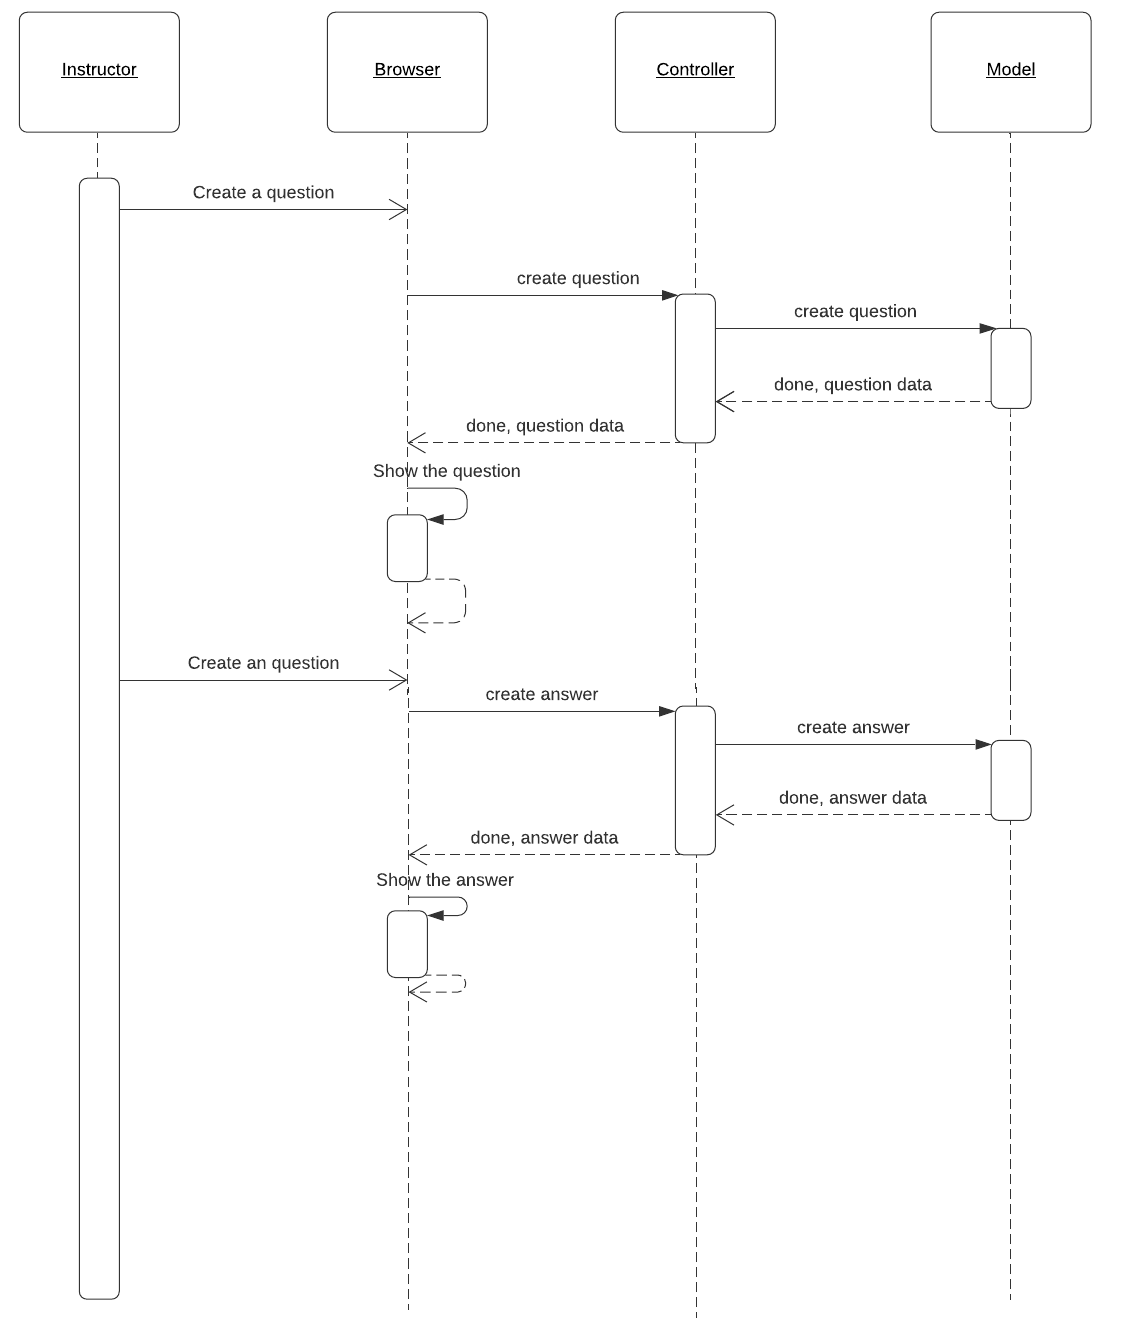
\includegraphics[width=142mm]{seq_create_exam.png}
    \caption{Sequence diagram of creating an exam}
    \label{fig:seq_create_exam}
\end{figure}


\vfill
\clearpage

%%%%%table
\begin{table}[H]
\centering
\caption{apply to become an instructor textual description}
\begin{tabular}{|p{4cm}|p{10cm}|}
\hline
\textbf{\large{Use case name}} & Recieve messages \\\hline
\textbf{\large{Actors}} & User \\\hline
\textbf{\large{Preconditions}} & User logged in \\\hline
\textbf{\large{Postconditions}} & Application sent \\\hline
\textbf{\large{Normal flow}} & 
\begin{itemize}
  \item The user visit the application form page.
  \item The user type the form data needed.
  \item The user submit the application.
\end{itemize}
\\\hline

\end{tabular}
\end{table}
%%%%%table

\begin{figure}[!ht]
    \centering
    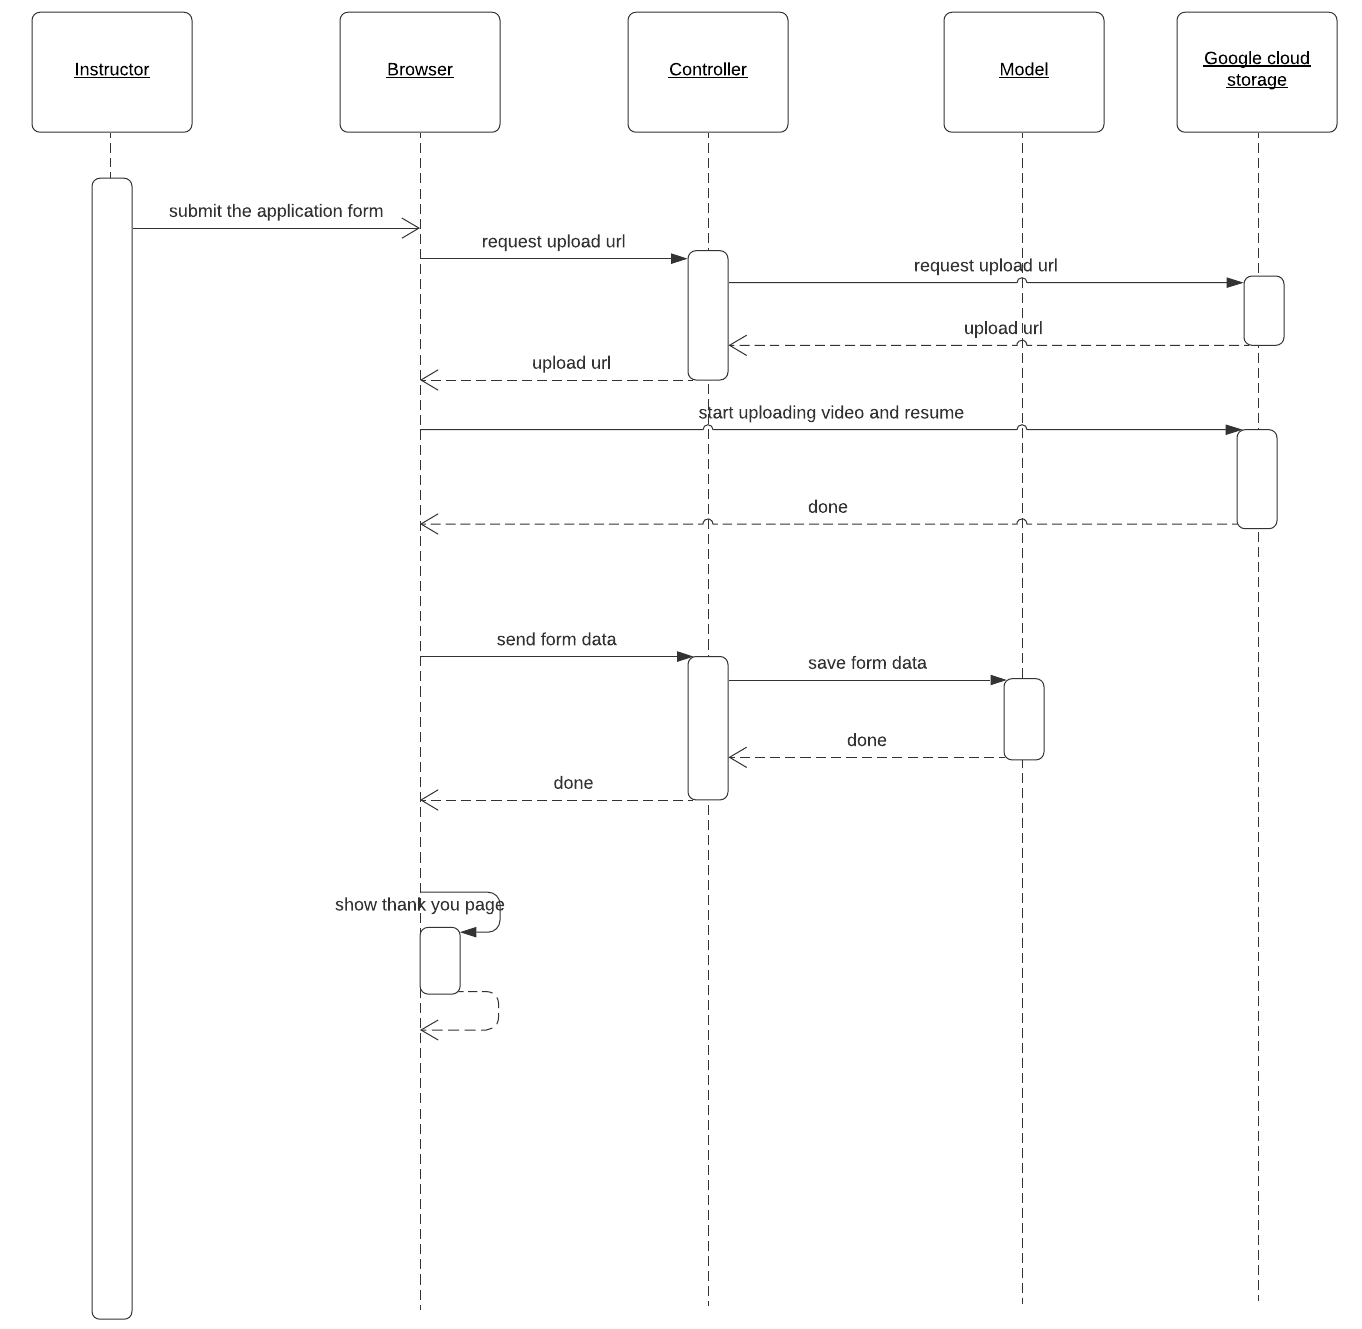
\includegraphics[width=150mm]{seq_apply_instructor.png}
    \caption{Sequence diagram of applying to become an instructor}
    \label{fig:seq_apply_instructor}
\end{figure}



\section{Implementation}
\subsection{Create an exam}
The instructor can manage and create an exam by clicking on the course and visiting the exam menu. An exam is composed of questions and questions have multiple answers and only one of them is correct.

To create a question, the instructor just needs type in the question and click add a question button which will fire a request to the server and in return we get the question data, we add that to the redux state to update the interface.

The user can also delete questions or answers which will make a request to delete the corresponding record and upon a successful request we remove the data the from redux state to update the interface.

\begin{figure}[!ht]
    \centering
    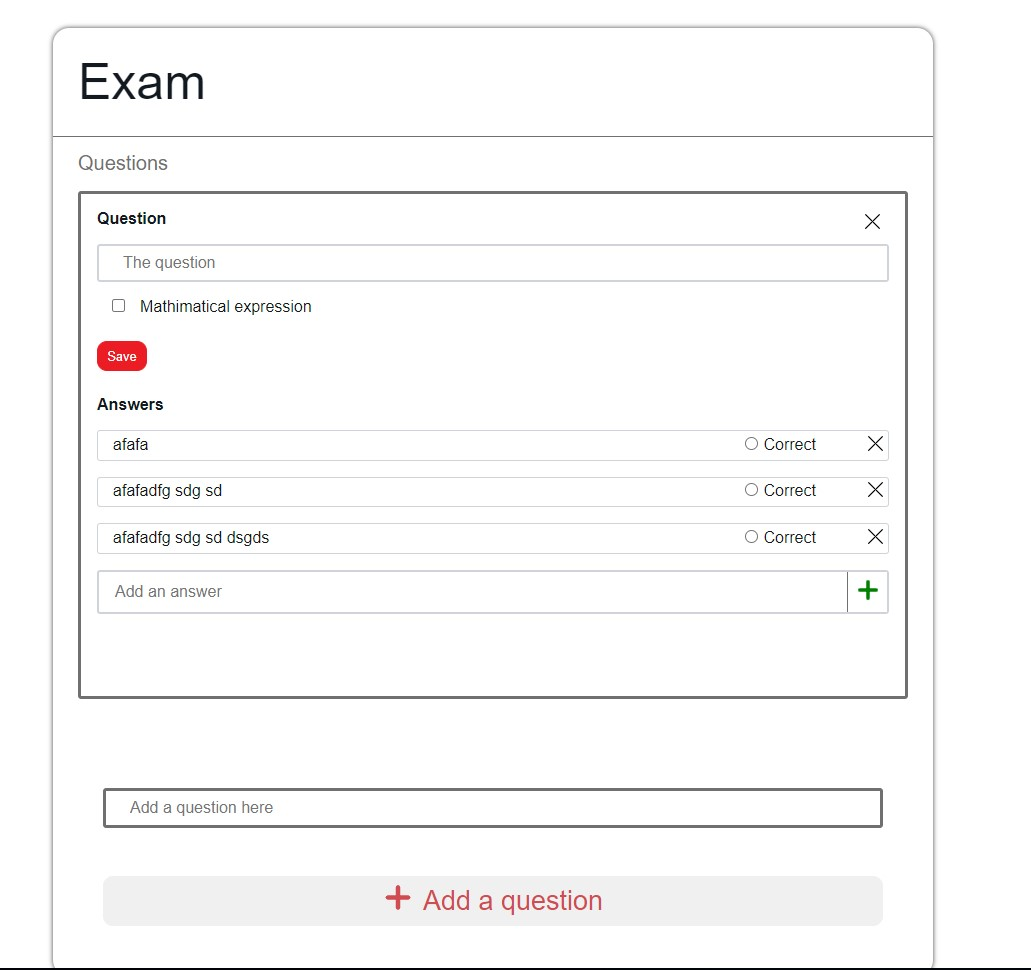
\includegraphics[width=150mm]{exam_form.jpg}
    \caption{Exam form interface}
    \label{fig:exam_form}
\end{figure}

\subsection{Apply to become an instructor}
If the current logged in user is not an instructor and tries to visit the instructor dashboard, he will be redirected to the instructor application form page.
When the user types the required form data and submits it, we request two upload url from the server and start uploading the cv and the video. Once it's done, we make a request to the server to save the submitted data.
\hfill \break
\hfill \break

\vfill
\clearpage

\begin{figure}[!ht]
    \centering
    
\includegraphics[width=150mm]{apply_instructor_1.jpg}
    \caption{Apply instructor page interface}
    \label{fig:apply_instructor_1}
\end{figure}


\hfill \break
\hfill \break
\hfill \break
\hfill \break

\begin{figure}[!ht]
    \centering
    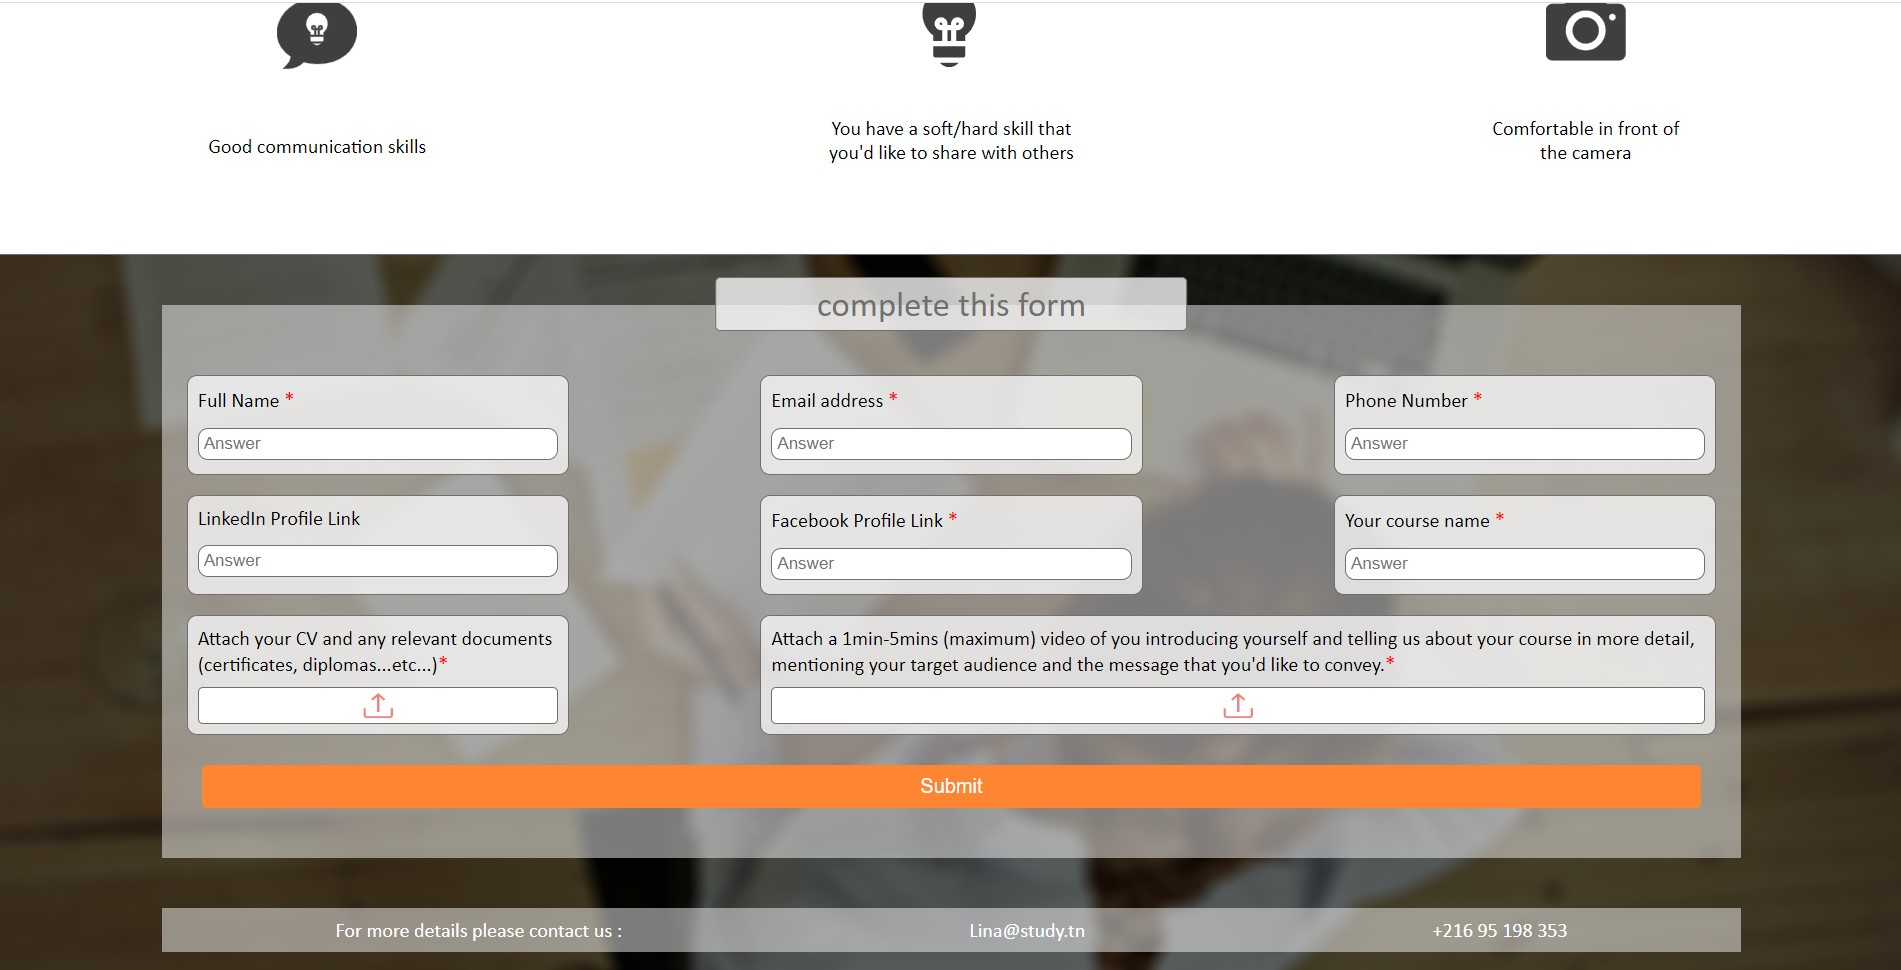
\includegraphics[width=150mm]{apply_instructor_2.jpg}
    \caption{Apply instructor form interface}
    \label{fig:apply_instructor_2}
\end{figure}


\vfill
\clearpage

\section*{Conclusion}
In this sprint, we have covered how the instructor can create an exam and how become an instructor.
\addcontentsline{toc}{section}{Conclusion}
\section*{General conclusion}
Through this report, I presented the work I did during my internship with
VIPAY SARL. The objective of the internship was the design and implementation of an insturctor dashboard for the website study.tn.

\hfill \break
\hfill \break
Regarding the approach, we first carried out a phase of analysing the existing tool. Second, we specified our application and it's major advantages compared to the existing solution. Thirdly, we proceeded to its modeling and design. Finally, we have implemented it.
\hfill \break
\hfill \break
This was a good learning experience, it allowed me to discover the different
web programming techniques associated with React as well as discovering the world of e-learning.
\nocite{*}
\bibliographystyle{unsrt}
\bibliography{references.bib}
\end{document}